%!TEX root = ../larxxia.tex


\section{Find eigenvalues and eigenvectors of matrices}
\label{sec:eennm}
\secttoc
\begin{comment}
\pooliv{\S4.3}  \layiv{\S5.2} \holti{\S6.1}  \cite[Ch.~9]{Chartier2015}
\end{comment}


Given the additional determinant methods of Chapter~\ref{ch:ddm}, this section begins exploring the properties and some applications of the eigen-problem \(A\xv=\lambda\xv\) for general matrices~\(A\).
We establish that there are generally \(n\)~eigenvalues of an \(n\times n\) matrix, albeit possibly complex valued, and that repeated eigenvalues are sensitive to errors.
Applications include population modelling, connecting to the computation of \svd{}s, and fitting exponentials to real data.




\subsection{A characteristic equation gives eigenvalues}
\label{sec:cege}

\begin{quoted}{J.~H. Wilkinson, 1984 \cite[p.103]{Higham1996}}
The Fundamental Theorem of Algebra asserts that every polynomial equation over the complex field has a root.  
It is almost beneath the dignity of such a majestic theorem to mention that in fact it has precisely \(n\)~roots.
\end{quoted}


Recall that eigenvalues~\(\lambda\) and non-zero eigenvectors~\xv\ of a square matrix~\(A\) must satisfy \((A-\lambda I)\xv=\ov\)\,.
Theorem~\ref{thm:detinv} then implies the \idx{eigenvalue}s of a \idx{square matrix} are precisely the solutions of the \bfidx{characteristic equation} \(\det(A-\lambda I)=0\)\,.  

\begin{theorem} \label{thm:geecp}
We call \(\det(A-\lambda I)\) the \bfidx{characteristic polynomial} of \idx{square matrix}~\(A\). 
\footnote{Alternatively, many call \(\det(\lambda I-A)\) the characteristic polynomial, as does \script.  
The distinction is immaterial as,  for an \(n\times n\) matrix~\(A\) and by Theorem~\ref{thm:basicdet:iii} with multiplicative factor \(k=-1\)\,, the only difference in the determinant is a factor of~\((-1)^n\).
In \script, \index{poly()@\texttt{poly()}}\texttt{poly(A)} computes the characteristic polynomial of the matrix,  \(\det(\lambda I-A)\), which might be useful for exercises, but is rarely useful in practice due to poor conditioning.} 
The characteristic polynomial of an \(n\times n\) matrix~\(A\) is a polynomial of \(n\)th~degree in~\(\lambda\).
Consequently, there are at most \(n\)~distinct eigenvalues of  an \(n\times n\) matrix~\(A\).
\end{theorem}

\begin{proof} 
% Do not do this as we want the induction for the next theorem's proof.
%Consider the characteristic polynomial
%\begin{equation*}
%\det(A-\lambda I)=
%\det\begin{bmatrix} a_{11}-\lambda&a_{12}&\cdots&a_{1n}
%\\a_{21}&a_{22}-\lambda&&a_{2n}
%\\\vdots&&\ddots&\vdots
%\\a_{n1}&a_{n2}&\cdots&a_{nn}-\lambda \end{bmatrix}.
%\end{equation*}
%Recall Theorem~\ref{thm:detnfac} asserts that the determinant of an \(n\times n\) matrix is a sum of \(n!\)~terms where each term is a product of \(n\)~factors where each factor in a term comes from a different row and column of the matrix.
%Being a sum of products of these entries, \(\det(A-\lambda I)\) is a polynomial in~\(\lambda\).
%Since each term is a product of \(n\)~factors, and each factor is an entry in the matrix~\(A-\lambda I\)\,, and each entry is at most linear in~\(\lambda\), then the polynomial is of degree at most~\(n\) in~\(\lambda\).
%One of the \(n!\)~terms in the sum is the product along the diagonal \((a_{11}-\lambda)(a_{22}-\lambda)\cdots(a_{nn}-\lambda)\): consequently the polynomial has a term in~\(\lambda^n\) and so is of degree~\(n\).
Use induction on the size of the matrix.
First, for \(1\times 1\) matrix \(A=\begin{bmatrix} a_{11} \end{bmatrix}\), the determinant \(\det(A-\lambda I)=\det \begin{bmatrix} a_{11}-\lambda \end{bmatrix}=a_{11}-\lambda\) which is of  degree one in~\(\lambda\).
Second, assume that for all \((n-1)\times (n-1)\) matrices~\(A\), \(\det(A-\lambda I)\) is a polynomial of degree~\(n-1\) in~\(\lambda\).
Then use the Laplace Expansion Theorem~\ref{thm:letdet} to give the first row expansion, in terms of minors of~\(A\) and~\(I\),
\begin{eqnarray*}
\det(A-\lambda I)
&=&(a_{11}-\lambda)\det (A_{11}-\lambda I_{11})
\\&&{}
-a_{12}\det (A_{12}-\lambda I_{12})
\\&&{}
+\cdots-(-1)^{n}a_{1n}\det (A_{1n}-\lambda I_{1n}).
\end{eqnarray*}
Now the minor~\(I_{11}\) is precisely the \((n-1)\times(n-1)\) identity, and hence by assumption \(\det(A_{11}-\lambda I_{11})\) is a polynomial of degree~\((n-1)\) in~\(\lambda\).
But differently, the minors~\(I_{12},\ldots,I_{1n}\) have two of the ones removed from the \(n\times n\)~identity and hence \(\lambda I_{12},\ldots,\lambda I_{1n}\) each have only \((n-2)\)~\(\lambda\)s: since each term in a determinant is a product of distinct entries of the matrix (Theorem~\ref{thm:detnfac}) it follows that for \(j\geq2\) the determinant \(\det(A_{1j}-\lambda I_{1j})\) is a polynomial in~\(\lambda\) of degree\({}\leq n-2\)\,.
Consequently, the first row expansion of 
\begin{eqnarray*}
\det(A-\lambda I)
&=&(a_{11}-\lambda)(\text{poly degree }n-1)
\\&&{}
-a_{12}(\text{poly degree }\leq n-2)
\\&&{}
+\cdots-(-1)^{n}a_{1n}(\text{poly degree }\leq n-2)
\\&=&(a_{11}-\lambda)(\text{poly degree }n-1)
\\&&{}
+(\text{poly degree }\leq n-2)
\\&=&(\text{poly degree }n)
\end{eqnarray*}
as the highest power of~\(\lambda\) cannot be cancelled by any term.
Induction thus implies the characteristic polynomial of an \(n\times n\) matrix~\(A\) is a polynomial of \(n\)th~degree in~\(\lambda\).

Lastly, because the characteristic polynomial of~\(A\) is of \(n\)th~degree in~\(\lambda\), the Fundamental Theorem of Algebra asserts that the polynomial has at most \(n\)~roots (possibly complex).  
Hence there are at most \(n\)~distinct eigenvalues.
\end{proof}



\begin{example} \label{eg:}
Find the \idx{characteristic polynomial} of each of the following matrices.  
Where in the coefficients of the polynomial can you see the determinant? and the sum of the diagonal elements?
\begin{enumerate}
\item \(\eAii=\begin{bmatrix} 1&-1\\-2&4 \end{bmatrix}\)
\begin{solution} 
The characteristic polynomial is \(\det(\eAii-\lambda I)
=\det\begin{bmatrix} 1-\lambda&-1\\-2&4-\lambda \end{bmatrix}
=(1-\lambda)(4-\lambda)-2
=\lambda^2-5\lambda+2\)\,.
Now \(\det \eAii=4-2=2\) which is the coefficient of the constant term in this polynomial.
Whereas the sum of the diagonal of~\(\eAii\) is \(1+4=5\) which is the negative of the \(\lambda\)~coefficient in the polynomial.
\end{solution}

\item \(\eAii=\begin{bmatrix}4&-2&1
\\1&-2&0
\\8&2&6 \end{bmatrix}\)
\begin{solution} 
The characteristic polynomial is 
\begin{eqnarray*}
\det(\eAii-\lambda I)
&=&\det\begin{bmatrix} 4-\lambda&-2&1
\\1&-2-\lambda&0
\\8&2&6-\lambda \end{bmatrix}
\\&=&(4-\lambda)(-2-\lambda)(6-\lambda)+0+2
\\&&{}
-(-2-\lambda)8-0-(-2)(6-\lambda)
\\&=&-48+4\lambda+8\lambda^2-\lambda^3+2
\\&&{}
+16+8\lambda+12+2\lambda
\\&=&-\lambda^3+8\lambda^2+2\lambda-18\,.
\end{eqnarray*}
Now \(\det \eAii=4(-2)6+0+2-(-2)8-0-(-2)6=-48+2+16+12=-18\) which is the coefficient of the constant term in the polynomial.
Whereas the sum of the diagonal of~\(\eAii\) is \(4-2+6=8\) which is the \(\lambda^2\)~coefficient in the polynomial.
\end{solution}

\end{enumerate}
\end{example}

These observations about the coefficients in the characteristic polynomials leads to the next theorem.

\begin{theorem} \label{thm:charpolyc}
For an \(n\times n\) matrix~\(A\), the product of the \idx{eigenvalue}s equals~\(\det A\) and equals the \idx{constant term} in the \idx{characteristic polynomial}.  
\begin{aside}
This optional theorem helps establish the nature of a characteristic polynomial.
\end{aside}
The sum of the \idx{eigenvalue}s equals \((-1)^{n-1}\)~times the \idx{coefficient} of~\(\lambda^{n-1}\) in the \idx{characteristic polynomial} and equals the \bfidx{trace} of the matrix, \(a_{11}+a_{22}+\cdots+a_{nn}\)\,.
% that is, \(\sum_{j=1}^n a_{jj}\).
\end{theorem}

\begin{proof} 
Theorem~\ref{thm:geecp}, and its proof, establishes that the characteristic polynomial has the form
\begin{eqnarray}
\det(A-\lambda I)&=&c_0+c_1\lambda+\cdots+c_{n-1}\lambda^{n-1}+(-1)^n\lambda^n
\nonumber\\&=&(\lambda_1-\lambda)(\lambda_2-\lambda)\cdots(\lambda_n-\lambda),
\label{eq:charpolyc}
\end{eqnarray}
where the second equality follows from the Fundamental Theorem of Algebra that an \(n\)th~degree polynomial factors into \(n\)~linear factors (albeit possibly complex).
First, substitute \(\lambda=0\) and this equation~\eqref{eq:charpolyc} gives \(\det A=c_0=\lambda_1\lambda_2\cdots\lambda_n\)\,, as required.

Second, consider the term~\(c_{n-1}\lambda^{n-1}\) in equation~\eqref{eq:charpolyc}.
From the factorisation on the right-hand side, the \(\lambda^{n-1}\)~term arises as
\begin{eqnarray*}
c_{n-1}\lambda^{n-1}&=&\lambda_1(-\lambda)^{n-1}
+(-\lambda)\lambda_2(-\lambda)^{n-2}
+\cdots+(-\lambda)^{n-1}\lambda_n
\\&=&(-1)^{n-1}(\lambda_1+\lambda_2+\cdots+\lambda_n)\lambda^{n-1},
\end{eqnarray*}
and hence the coefficient \(c_{n-1}=(-1)^{n-1}(\lambda_1+\lambda_2+\cdots+\lambda_n)\), as required.
Now use induction to prove the trace formula.
Recall that the proof of Theorem~\ref{thm:geecp} establishes that
\begin{eqnarray*}
\det(A-\lambda I)
&=&(a_{11}-\lambda)\det (A_{11}-\lambda I_{11})
\\&&{}
+(\text{poly degree }\leq n-2).
\end{eqnarray*}
Assume the trace formula holds for \((n-1)\times(n-1)\) matrices such as the minor~\(A_{11}\). Then the previous identity gives
\begin{eqnarray*}
\det(A-\lambda I)
&=&(a_{11}-\lambda)\big[(-1)^{n-1}\lambda^{n-1}
\\&&\quad{}
+(-1)^{n-2}(a_{22}+\cdots+a_{nn})\lambda^{n-2} 
\\&&\quad{}
+(\text{poly degree }\leq n-3)\big]
\\&&{}
+(\text{poly degree }\leq n-2)
\\&=&(-1)^{n}\lambda^{n}
%\\&&{}
+(-1)^{n-1}(a_{11}+a_{22}+\cdots+a_{nn})\lambda^{n-1} 
\\&&{}
+(\text{poly degree }\leq n-2).
\end{eqnarray*}
Hence the coefficient \(c_{n-1}=(-1)^{n-1}(a_{11}+a_{22}+\cdots+a_{nn})\).
Since the formula holds for the basic case \(n=1\), namely \(c_0=+a_{11}\)\,, induction implies the sum of the eigenvalues
\(\lambda_1+\lambda_2+\cdots+\lambda_n=a_{11}+a_{22}+\cdots+a_{nn}\)\,, the trace of the matrix~\(A\).
\end{proof}



\begin{example} \label{eg:}
\begin{enumerate}
\item What are the two highest order terms and the constant term in the \idx{characteristic polynomial} of the matrix
\begin{equation*}
\eAii=\begin{bmatrix}-2&-1&3&-2
\\-1&3&-2&2
\\2&-3&0&1
\\0&1&0&-3  \end{bmatrix}.
\end{equation*}
\begin{solution} 
First compute the determinant using the Laplace expansion (Theorem~\ref{thm:letdet}).  
The two zeros in the last row suggest a last row expansion:
\begin{eqnarray*}
\det \eAii&=&(-1)^61\det\begin{bmatrix}-2&3&-2
\\-1&-2&2
\\2&0&1 \end{bmatrix}
\\&&{}
+(-1)^8(-3)\det\begin{bmatrix}-2&-1&3
\\-1&3&-2
\\2&-3&0\end{bmatrix}
\\&=&(4+12+0-8-0+3)
\\&&{}-3(0+4+9-18+12-0)
=-10\,.
\end{eqnarray*}
This is the constant term in the characteristic polynomial.
Second, the trace of~\(\eAii\) is \(-2+3+0-3=-2\) so the cubic coefficient in the characteristic polynomial is~\((-1)^3(-2)=2\)\,.
That is, the characteristic polynomial of~\(\eAii\) is of the form \(\lambda^4+2\lambda^3+\cdots-10\)\,.
\end{solution}

\item After laborious calculation you find the \idx{characteristic polynomial} of the matrix
\begin{equation*}
\eAii=\begin{bmatrix}-2&5&-3&-1&2
\\-2&-5&-1&-1&3
\\1&4&-2&1&-7
\\1&-5&1&4&-5
\\-1&0&3&-3&1\end{bmatrix}
\end{equation*}
is \(-\lambda^5+2\lambda^4-3\lambda^3+234\lambda^2+884\lambda+1564\)\,.  
Could this polynomial be correct?
\begin{solution} 
No, because the trace of~\(\eAii\) is \(-2-5-2+4+1=-4\) so the coefficient of the \(\lambda^4\)~term must be~\((-1)^4(-4)=-4\) instead of the calculated~\(2\).
\end{solution}

\item After much calculation you find the \idx{characteristic polynomial} of the matrix
\begin{equation*}
\eAii=\begin{bmatrix}0&0&3&1&0&0
\\0&0&0&0&0&1
\\0&0&-4&0&3&0
\\-5&0&3&0&0&0
\\0&0&0&0&0&2
\\0&0&0&-6&0&0\end{bmatrix}
\end{equation*}
is \(\lambda^6 +4\lambda^5 +5\lambda^4 +20\lambda^3 +108\lambda^2 -540\lambda+668\)\,.  
Could this polynomial be correct?
\begin{solution} 
No. By the column of zeros in~\(\eAii\), \(\det \eAii\) must be zero instead of the calculated~\(668\).
\end{solution}

\item What are the two highest order terms and the constant term in the \idx{characteristic polynomial} of the matrix
\begin{equation*}
\eAii=\begin{bmatrix}0&4&0&0&3&0
\\-2&0&0&1&0&-2
\\0&0&0&-1&0&0
\\0&0&-5&0&-4&3
\\0&2&-3&0&-4&0
\\0&-3&0&0&0&0\end{bmatrix}.
\end{equation*}
\begin{solution} 
First compute the determinant using the Laplace expansion (Theorem~\ref{thm:letdet}).  
The nearly all zeros in the last row suggests starting with a last row expansion (although others are just as good):
\begin{eqnarray*}
\det \eAii&=&(-1)^8(-3)\det\begin{bmatrix}0&0&0&3&0
\\-2&0&1&0&-2
\\0&0&-1&0&0
\\0&-5&0&-4&3
\\0&-3&0&-4&0\end{bmatrix}
\\&&(\text{using a 3rd row expansion})
\\&=&-3(-1)^6(-1)\det\begin{bmatrix}0&0&3&0
\\-2&0&0&-2
\\0&-5&-4&3
\\0&-3&-4&0\end{bmatrix}
\\&&(\text{using a 1st column expansion})
\\&=&3(-1)^3(-2)\det\begin{bmatrix}0&3&0
\\-5&-4&3
\\-3&-4&0\end{bmatrix}
\\&&(\text{using a 3rd column expansion})
\\&=&6(-1)^53\det\begin{bmatrix}0&3
\\-3&-4\end{bmatrix}
\\&=&-18(0+9)=-162\,.
\end{eqnarray*}
This is the constant term in the characteristic polynomial.
Second, the trace of~\(\eAii\) is \(0+0+0+0-4+0=-4\) so the quintic coefficient in the characteristic polynomial is~\((-1)^5(-4)=4\)\,.
That is, the characteristic polynomial of~\(\eAii\) is of the form \(\lambda^6+4\lambda^5+\cdots-162\)\,.
\end{solution}

\end{enumerate}
\end{example}






\begin{definition} \label{def:eigmult}
An \idx{eigenvalue}~\(\lambda_0\) of a matrix~\(A\) is said to have \bfidx{multiplicity}~\(m\) if the \idx{characteristic polynomial} factorises to \(\det(A-\lambda I)=(\lambda-\lambda_0)^mg(\lambda)\) where \(g(\lambda_0)\neq0\)\,, and \(g(\lambda)\)~is a polynomial of degree~\(n-m\)\,.
Any eigenvalue of multiplicity \(m\geq2\) is also called a \bfidx{repeated eigenvalue}.
\end{definition}



\begin{example} \label{eg:faem}
Use the \idx{characteristic polynomial} to find all \idx{eigenvalue}s and their \idx{multiplicity} of the following matrices.
\begin{enumerate}
\item\label{eg:faem:a} \(\eAii=\begin{bmatrix} 3&1\\0&3 \end{bmatrix}\)
\begin{solution}The characteristic equation is \(\det(\eAii-\lambda I)
=\det{\small\begin{bmatrix} 3-\lambda&1\\0&3-\lambda \end{bmatrix}}
=(3-\lambda)^2-0\cdot1=(\lambda-3)^2=0\). 
The only eigenvalue is \(\lambda=3\) with multiplicity two.
(Since this is an upper triangular matrix, the eigenvalues are the diagonal elements, namely~\(3\) twice.)
\end{solution}

\item\label{eg:faem:b} \(\eAii=\begin{bmatrix}-1&1&-2
\\-1&0&-1
\\0&-3&1 \end{bmatrix}\)
\begin{solution}The characteristic equation is 
\begin{eqnarray*}
\det(\eAii-\lambda I)
&=&\det\begin{bmatrix}-1-\lambda&1&-2
\\-1&-\lambda&-1
\\0&-3&1-\lambda\end{bmatrix}
\\&=&(1+\lambda)\lambda(1-\lambda)+0-6
\\&&{}
-0+3(1+\lambda)+(1-\lambda)
\\&=&-\lambda^3+3\lambda-2
\\&=&-(\lambda-1)^2(\lambda+2)=0\,.
\end{eqnarray*}
Eigenvalues are \(\lambda=1\) with multiplicity two, and \(\lambda=-2\) with multiplicity one.
\end{solution}


\item\label{eg:faem:c} \(\eAii=\begin{bmatrix}-1&0&-2
\\0&-3&2
\\0&-2&1\end{bmatrix}\)
\begin{solution}The characteristic equation is 
\begin{eqnarray*}
\det(\eAii-\lambda I)
&=&\det\begin{bmatrix}-1-\lambda&0&-2
\\0&-3-\lambda&2
\\0&-2&1-\lambda\end{bmatrix}
\\&=&(-1-\lambda)\det\begin{bmatrix} -3-\lambda&2
\\-2&1-\lambda \end{bmatrix}
\\&=&-(1+\lambda)\big[(-3-\lambda)(1-\lambda)+4\big]
\\&=&-(\lambda+1)\big[\lambda^2+2\lambda+1\big]
\\&=&-(\lambda+1)^3=0\,.
\end{eqnarray*}
The only eigenvalue is \(\lambda=-1\) with multiplicity three.
\end{solution}

\item \(\eAii=\begin{bmatrix}2&0&-1
\\-5&3&-5
\\5&-2&-2\end{bmatrix}\)
\begin{solution}The characteristic equation is 
\begin{eqnarray*}
\det(\eAii-\lambda I)
&=&\det\begin{bmatrix}2-\lambda&0&-1
\\-5&3-\lambda&-5
\\5&-2&-2-\lambda\end{bmatrix}
\\&=&(2-\lambda)(3-\lambda)(-2-\lambda)+0-10
\\&&{}
+5(3-\lambda)-10(2-\lambda)-0
\\&=&-\lambda^3+3\lambda^2+9\lambda-27
\\&=&-(\lambda-3)^2(\lambda+3)=0\,.
\end{eqnarray*}
Eigenvalues are \(\lambda=3\) with multiplicity two, and \(\lambda=-3\) with multiplicity one.
\end{solution}

\item \(E=\begin{bmatrix} 0&1\\-1&1 \end{bmatrix}\)
\begin{solution} 
The characteristic equation is
\begin{eqnarray*}
\det(E-\lambda I)
&=&\det\begin{bmatrix} -\lambda&1\\-1&1-\lambda \end{bmatrix}
\\&=&-\lambda(1-\lambda)+1
\\&=&\lambda^2-\lambda+1=0\,.
\end{eqnarray*}
This quadratic equation does not factor easily so use the formula 
\begin{equation*}
\lambda=\frac{-b\pm\sqrt{b^2-4ac}}{2a}
=\frac{1\pm\sqrt{1-4}}{2}
%=\tfrac12(1\pm\sqrt{-3})
=\frac12\pm\frac{\sqrt3}2i\,,
\end{equation*}
for \(i=\sqrt{-1}\), are two eigenvalues (complex valued) each of multiplicity one.
\end{solution}

\end{enumerate}
\end{example}


%\begin{verbatim}
%for i=1:99999,a=round(randn(4)*3);l=eig(a);if min(abs(diff(l)))<1e-6,a=a,lam=l,break,end,end
%\end{verbatim}


\begin{example} \label{eg:multeval}
Use \index{eig()@\texttt{eig()}}\verb|eig()| in \script\  to find the \idx{eigenvalue}s and their multiplicity for the following matrices.
Recall (Table~\ref{tbl:mtlbeig}) that executing just \verb|eig(A)| gives a column vector of eigenvalues of~\(A\), repeated according to their \idx{multiplicity}. 
\begin{enumerate}
\item \(\begin{bmatrix}2&2&-1
\\0&1&-2
\\0&-1&0\end{bmatrix}\)
\begin{solution} 
Execute \verb|eig([2 2 -1;0 1 -2;0 -1 0])| to get
\setbox\ajrqrbox\hbox{\qrcode{% eigenvalue code
eig([2 2 -1;0 1 -2;0 -1 0])
}}%
\marginpar{\usebox{\ajrqrbox}}%
\begin{verbatim}
ans =
   2
   2
  -1
\end{verbatim}
So the eigenvalue \(\lambda=2\) has multiplicity two, and the eigenvalue \(\lambda=-1\) has multiplicity one.
\end{solution}

\item \(\begin{bmatrix}-2&-2&-5&0
\\0&-2&2&1
\\-1&1&0&-1
\\-2&1&4&0\end{bmatrix}\)
\begin{solution} 
In \script\ execute
\begin{verbatim}
eig([-2 -2 -5 0
  0 -2 2 1
 -1 1 0 -1
 -2 1 4 0])
\end{verbatim}
\setbox\ajrqrbox\hbox{\qrcode{% eigenvalue code
eig([-2 -2 -5 0
  0 -2 2 1
 -1 1 0 -1
 -2 1 4 0])
}}%
\marginpar{\usebox{\ajrqrbox}}%
to get
\begin{verbatim}
ans =
  -3.0000 + 0.0000i
  -3.0000 + 0.0000i
   1.0000 + 1.4142i
   1.0000 - 1.4142i
\end{verbatim}
There are two complex-valued eigenvalues, evidently \(1\pm\sqrt2i\), each of multiplicity one, and also the (real) eigenvalue \(\lambda=-3\) which has multiplicity two.
\end{solution}

\item \(\begin{bmatrix}3&-1&-2&1&-2
\\0&0&-2&-2&0
\\2&1&1&1&-1
\\-1&-3&0&1&2
\\2&-2&1&0&3\end{bmatrix}\)
\begin{solution} 
In \script\ execute
\begin{verbatim}
eig([3 -1 -2 1 -2
  0 0 -2 -2 0
  2 1 1 1 -1
 -1 -3 0 1 2
  2 -2 1 0 3])
\end{verbatim}
\setbox\ajrqrbox\hbox{\qrcode{% eigenvalue code
eig([3 -1 -2 1 -2
  0 0 -2 -2 0
  2 1 1 1 -1
 -1 -3 0 1 2
  2 -2 1 0 3])
}}%
\marginpar{\usebox{\ajrqrbox}}%
to get
\begin{verbatim}
ans =
   2.0000 + 2.8284i
   2.0000 - 2.8284i
   4.0000 + 0.0000i
  -0.0000 + 0.0000i
  -0.0000 - 0.0000i
\end{verbatim}
There are three eigenvalues of multiplicity one, namely \(4\) and \(2\pm\sqrt8i\)\,.  
The last two rows appear to be the eigenvalue \(\lambda=0\) with multiplicity two.
\end{solution}

\item \(\begin{bmatrix}-1&0&0&0
\\-1&2&-3&3
\\3&1&-1&0
\\0&3&-2&1\end{bmatrix}\)
\begin{solution} 
In \script\ execute
\begin{verbatim}
eig([-1 0 0 0
 -1 2 -3 3
  3 1 -1 0
  0 3 -2 1])
\end{verbatim}
\setbox\ajrqrbox\hbox{\qrcode{% eigenvalue code
eig([-1 0 0 0
 -1 2 -3 3
  3 1 -1 0
  0 3 -2 1])
}}%
\marginpar{\usebox{\ajrqrbox}}%
to get
\begin{verbatim}
ans =
   4.0000 + 0.0000i
  -1.0000 + 0.0000i
  -1.0000 - 0.0000i
  -1.0000 + 0.0000i
\end{verbatim}
There is one eigenvalue of multiplicity one, \(\lambda=4\).  
The last three rows appear to be the eigenvalue \(\lambda=-1\) with multiplicity three.
\end{solution}

\end{enumerate}
\end{example}





To find eigenvalues and eigenvectors, the following restates Procedure~\ref{pro:eeh} with a little more information, and now empowered to address larger matrices with the determinant tools from Chapter~\ref{ch:ddm}.

\begin{procedure}[eigenvalues and eigenvectors] \label{pro:geneig}
To find by hand \idx{eigenvalue}s and \idx{eigenvector}s of a (small) \idx{square matrix}~\(A\):
\begin{enumerate}
%\item determine the \idx{characteristic polynomial} of~\(A\), \(\det(A-\lambda I)\);
\item find all \idx{eigenvalue}s (possibly complex) by solving the \bfidx{characteristic equation} of~\(A\), \(\det(A-\lambda I)=0\)\,;
\item for each \idx{eigenvalue}~\(\lambda\), solve \((A-\lambda I)\xv=\ov\) to find the \idx{eigenspace}~\(\EE_\lambda\) of all \idx{eigenvector}s (together with~\ov);
\item write each eigenspace as the \idx{span} of a few chosen \idx{eigenvector}s  (Definition~\ref{def:basis} calls such a set a \idx{basis}).
\end{enumerate}
Since, for an \(n\times n\) matrix, the \idx{characteristic polynomial} is of \(n\)th~degree in~\(\lambda\) (Theorem~\ref{thm:geecp}), there are \(n\)~\idx{eigenvalue}s (when counted according to \idx{multiplicity} and allowing \idx{complex eigenvalue}s).
\end{procedure}

Correspondingly, the following restates the computational procedure of section~\ref{sec:cee}, but slightly more generally: the extra generality caters for non-symmetric matrices.

\begin{compute}
For a given square matrix~\verb|A|, execute \verb|[V,D]=eig(A)|, then the diagonal entries of~\verb|D|, \verb|diag(D)|, are the \idx{eigenvalue}s of~\verb|A|. 
Corresponding to the eigenvalue~\verb|D(j,j)| is an  \idx{eigenvector} \(\vv_j=\verb|V(:,j)|\), the \(j\)th~column of~\verb|V|.  
\footnote{Be aware that \script\ does not use the determinant to find the eigenvalues, nor does it solve the linear equations to find eigenvectors.  
For any but the smallest matrices such a `by hand' approach is far too expensive.  
Instead, to find eigenvalues and eigenvectors, just as for the \svd, \script\ uses an intriguing iteration based upon what is called the \idx{QR factorisation}\ifcsname ch:qrfuma\endcsname\ (Chapter~\ref{ch:qrfuma})\fi.}
If an \idx{eigenvalue} is repeated (multiplicity more than one), then the corresponding columns of~\verb|V| span the \idx{eigenspace} (and, as Section~\ref{sec:lisb} discusses, the column vectors are a so-called \idx{basis} for the eigenspace when they have a property called \idx{linear independence}). 
\end{compute}


\begin{example} \label{eg:faespm}
Find the eigenspaces corresponding to the eigenvalues found for the first three matrices of Example~\ref{eg:faem}.
\begin{itemize}
\item[\ref{eg:faem:a}.]
\(A=\begin{bmatrix} 3&1\\0&3 \end{bmatrix}\)
\begin{solution} 
The only eigenvalue is \(\lambda=3\) with multiplicity two.
Its eigenvectors~\xv\ satisfy
\begin{equation*}
(A-3 I)\xv=\begin{bmatrix} 0&1\\0&0 \end{bmatrix}\xv=\ov\,.
\end{equation*}
The second component of this equation is the trivial \(0=0\)\,.  The first component of the equation is \(0x_1+1x_2=0\), hence \(x_2=0\)\,.
All eigenvectors are of the form \(\xv=(1,0)x_1\)\,.  
That is the eigenspace  \(\EE_3=\Span\{(1,0)\}\).

In \script, executing \verb|[V,D]=eig([3 1;0 3])| gives us
\begin{verbatim}
V =
   1.0000  -1.0000
   0.0000   0.0000
D =
   3   0
   0   3
\end{verbatim}
Diagonal matrix~\verb|D| confirms the only eigenvalue is three, whereas the two columns of~\verb|V| confirm the eigenspace \(\EE_1=\Span\{(1,0),(-1,0)\}=\Span\{(1,0)\}\).
\end{solution}


\item[\ref{eg:faem:b}.]
\(B=\begin{bmatrix}-1&1&-2
\\-1&0&-1
\\0&-3&1 \end{bmatrix}\)
\begin{solution} 
The eigenvalues are \(\lambda=-2\) (multiplicity one) and \(\lambda=1\) (multiplicity two).
\begin{itemize}
\item For \(\lambda=-2\) solve
\begin{equation*}
(B+2I)\xv=\begin{bmatrix}1&1&-2
\\-1&2&-1
\\0&-3&3 \end{bmatrix}\xv=\ov\,.
\end{equation*}
The third component of this equation requires \(-3x_2+3x_3=0\)\,, that is, \(x_2=x_3\)\,.
The second component requires \(-x_1+2x_2-x_3=0\)\,, that is, \(x_1=2x_2-x_3=2x_3-x_3=x_3\)\,.
The first component requires \(x_1+x_2-2x_3=0\) which is also satisfied by \(x_1=x_2=x_3\)\,.
All eigenvectors are of the form \(x_3(1,1,1)\).
That is, the eigenspace \(\EE_{-2}=\Span\{(1,1,1)\}\).

\item For \(\lambda=1\) solve
\begin{equation*}
(B-1I)\xv=\begin{bmatrix}-2&1&-2
\\-1&-1&-1
\\0&-3&0 \end{bmatrix}\xv=\ov\,.
\end{equation*}
The third component of this equation requires \(-3x_2=0\)\,, that is, \(x_2=0\)\,.
The second component requires \(-x_1-x_2-x_3=0\)\,, that is, \(x_1=-x_2-x_3=0-x_3=-x_3\)\,.
The first component requires \(-2x_1+x_2-2x_3=0\) which is also satisfied by \(x_1=-x_3\) and \(x_2=0\).
All eigenvectors are of the form \(x_3(-1,0,1)\).
That is, the eigenspace \(\EE_{1}=\Span\{(-1,0,1)\}\).
\end{itemize}

Alternatively, in \script, executing 
\begin{verbatim}
B=[-1 1 -2
 -1 0 -1
 0 -3 1]
[V,D]=eig(B)
\end{verbatim}
gives us
\begin{verbatim}
V =
    -0.5774     0.7071    -0.7071
    -0.5774     0.0000     0.0000
    -0.5774    -0.7071     0.7071
D =
         -2          0          0
          0          1          0
          0          0          1
\end{verbatim}
Diagonal matrix~\verb|D| confirms the eigenvalues. 
The first column of~\verb|V| confirms the eigenspace 
\begin{eqnarray*}
\EE_{-2}&=&\Span\{(-0.5774,-0.5774,-0.5774)\}
\\&=&\Span\{(1,1,1)\}.
\end{eqnarray*}
Whereas the last two columns of~\verb|V| confirm the eigenspace 
\begin{eqnarray*}
\EE_1&=&\Span\{(0.7071,0,-0.7071),(-0.7071,0,0.7071)\}
\\&=&\Span\{(-1,0,1)\}.
\end{eqnarray*}
\end{solution}

\item[\ref{eg:faem:c}.]
\(C=\begin{bmatrix}-1&0&-2
\\0&-3&2
\\0&-2&1\end{bmatrix}\)
\begin{solution} 
The only eigenvalue is \(\lambda=-1\) with multiplicity three.
Its eigenvectors~\xv\ satisfy
\begin{equation*}
(C+1 I)\xv=\begin{bmatrix} 0&0&-2
\\0&-2&2
\\0&-2&2 \end{bmatrix}\xv=\ov\,.
\end{equation*}
The first component of this equation requires \(x_3=0\)\,.  
The second and third components both requires \(-2x_2+2x_3=0\), hence \(x_2=x_3=0\)\,.
Since \(x_1\) is unconstrained, all eigenvectors are of the form \(\xv=x_1(1,0,0)\).  
That is the eigenspace  \(\EE_{-1}=\Span\{(1,0,0)\}\).

Alternatively, in \script, executing 
\begin{verbatim}
C=[-1 0 -2
 0 -3 2
 0 -2 1]
[V,D]=eig(C)
\end{verbatim}
gives us
\begin{verbatim}
V =
           1          -1          -1
           0           0           0
           0           0           0
D =
          -1           0           0
           0          -1           0
           0           0          -1
\end{verbatim}
Diagonal matrix~\verb|D| confirms the only eigenvalue is one with multiplicity three.  
The three columns of~\verb|V| confirm the eigenspace \(\EE_{-1}=\Span\{(1,0,0)\}\).
\end{solution}

\end{itemize}
\end{example}

The matrices in Example~\ref{eg:faespm} all have repeated eigenvalues.  
For these repeated eigenvalues the corresponding eigenspaces were all one dimensional.
This contrasts with the case of symmetric matrices where the eigenspaces always have the same dimensionality as the multiplicity of the eigenvalue, as illustrated by Examples~\ref{eg:espace2d} and~\ref{eg:sier2eig}.
Subsequent sections work towards Theorem~\ref{thm:dimee} which establishes that for non-symmetric matrices an eigenspace has dimensionality between one and the multiplicity of the corresponding eigenvalue.


\begin{example} \label{eg:fiveev}
By hand, find the eigenvalues and eigenspaces of the matrix
\begin{equation*}
A=\begin{bmatrix}0&3&0&0&0
\\1&0&3&0&0
\\0&1&0&3&0
\\0&0&1&0&3
\\0&0&0&1&0\end{bmatrix}
\end{equation*}
Confirm your answer with \verb|eig()| in \script.
\begin{solution} 
Adopt Procedure~\ref{pro:geneig}.
\begin{enumerate}
\item The characteristic equation is
\begin{eqnarray*}
&&\det(A-\lambda I)
\\&=&\begin{vmatrix}-\lambda&3&0&0&0
\\1&-\lambda&3&0&0
\\0&1&-\lambda&3&0
\\0&0&1&-\lambda&3
\\0&0&0&1&-\lambda\end{vmatrix}
\\&&(\text{by first row expansion~\eqref{eq:detlet}})
\\&=&(-\lambda)\begin{vmatrix}-\lambda&3&0&0
\\1&-\lambda&3&0
\\0&1&-\lambda&3
\\0&0&1&-\lambda\end{vmatrix}
-3\begin{vmatrix}1&3&0&0
\\0&-\lambda&3&0
\\0&1&-\lambda&3
\\0&0&1&-\lambda\end{vmatrix}
\\&&(\text{by first row and first column expansion, respectively})
\\&=&(-\lambda)^2\begin{vmatrix}-\lambda&3&0
\\1&-\lambda&3
\\0&1&-\lambda\end{vmatrix}
-(-\lambda)3\begin{vmatrix}1&3&0
\\0&-\lambda&3
\\0&1&-\lambda\end{vmatrix}
\\&&{}
-3\begin{vmatrix}-\lambda&3&0
\\1&-\lambda&3
\\0&1&-\lambda\end{vmatrix}
\\&&(\text{by common factor, and first column expansion})
\\&=&(\lambda^2-3)\begin{vmatrix}-\lambda&3&0
\\1&-\lambda&3
\\0&1&-\lambda\end{vmatrix}
+3\lambda\begin{vmatrix}-\lambda&3
\\1&-\lambda\end{vmatrix}
\\&&(\text{using~\eqref{eq:dets23b}})
\\&=&(\lambda^2-3)\big[(-\lambda)^3+0+0-0+3\lambda+3\lambda\big]
+3\lambda(\lambda^2-3)
\\&=&(\lambda^2-3)(-\lambda^3+9\lambda)
\\&=&-\lambda(\lambda^2-3)(\lambda^2-9)=0\,.
\end{eqnarray*}
The five eigenvalues are thus \(\lambda=0,\pm\sqrt3,\pm3\)\,, all of multiplicity one.

\item Consider each eigenvalue in turn.
\begin{itemize}
\item[\(\lambda=0\)]  Solve
\begin{equation*}
(A-0I)\xv=\begin{bmatrix}0&3&0&0&0
\\1&0&3&0&0
\\0&1&0&3&0
\\0&0&1&0&3
\\0&0&0&1&0\end{bmatrix}\xv=\ov\,.
\end{equation*}
The last row requires \(x_4=0\)\,.
The fourth row requires \(x_3+3x_5=0\)\,, that is, \(x_3=-3x_5\)\,.
The third row requires \(x_2+3x_4=0\)\,, that is, \(x_2=-3x_4=-3\cdot 0=0\)\,.
The second row requires \(x_1+3x_3=0\)\,, that is, \(x_1=-3x_3=9x_5\)\,.
The first row requires \(3x_2=0\)\,, which is satisfied as \(x_2=0\)\,.
Since all eigenvectors are of the form \((9x_5,0,-3x_5,0,x_5)\), the eigenspace \(\EE_0=\Span\{(9,0,-3,0,1)\}\).

\item[\(\lambda=\pm\sqrt3\)]  Being careful with the upper and lower signs, solve \((A\mp\sqrt3I)\xv=\ov\)\,, that is,
\begin{equation*}
\begin{bmatrix}\mp\sqrt3&3&0&0&0
\\1&\mp\sqrt3&3&0&0
\\0&1&\mp\sqrt3&3&0
\\0&0&1&\mp\sqrt3&3
\\0&0&0&1&\mp\sqrt3\end{bmatrix}\xv=\ov\,.
\end{equation*}
The last row requires \(x_4\mp\sqrt3x_5=0\)\,, that is, \(x_4=\pm\sqrt3x_5\)\,.
The fourth row requires \(x_3\mp\sqrt3x_4+3x_5=0\)\,, that is, \(x_3=\pm\sqrt3x_4-3x_5=3x_5-3x_5=0\)\,.
The third row requires \(x_2\mp\sqrt3x_3+3x_4=0\)\,, that is, \(x_2=\pm\sqrt3x_3-3x_4=\mp3\sqrt3x_5\)\,.
The second row requires \(x_1\mp\sqrt3x_2+3x_3=0\)\,, that is, \(x_1=\pm\sqrt3x_2-3x_3=-9x_5\)\,.
The first row requires \(\mp\sqrt3x_1+3x_2=0\)\,, which is satisfied as \(\mp\sqrt3(-9x_5)+3(\mp3\sqrt3x_5)=0\)\,.
Since all eigenvectors are of the form \((-9x_5, \mp3\sqrt3x_5, 0, \pm\sqrt3x_5, x_5)\), the eigenspaces \(\EE_{\pm\sqrt3}=\Span\{(-9,\mp3\sqrt3,0,\pm\sqrt3,1)\}\).

\item[\(\lambda=\pm3\)]  Being careful with the upper and lower signs, solve \((A\mp3I)\xv=\ov\)\,, that is,
\begin{equation*}
\begin{bmatrix}\mp3&3&0&0&0
\\1&\mp3&3&0&0
\\0&1&\mp3&3&0
\\0&0&1&\mp3&3
\\0&0&0&1&\mp3\end{bmatrix}\xv=\ov\,.
\end{equation*}
The last row requires \(x_4\mp3x_5=0\)\,, that is, \(x_4=\pm3x_5\)\,.
The fourth row requires \(x_3\mp3x_4+3x_5=0\)\,, that is, \(x_3=\pm3x_4-3x_5=9x_5-3x_5=6x_5\)\,.
The third row requires \(x_2\mp3x_3+3x_4=0\)\,, that is, \(x_2=\pm3x_3-3x_4=\pm9x_5\)\,.
The second row requires \(x_1\mp3x_2+3x_3=0\)\,, that is, \(x_1=\pm3x_2-3x_3=9x_5\)\,.
The first row requires \(\mp3x_1+3x_2=0\)\,, which is satisfied as \(\mp3(9x_5)+3(\pm9x_5)=0\)\,.
Since all eigenvectors are of the form \((9x_5, \pm9 x_5, 6x_5, \pm3x_5, x_5)\), the eigenspaces \(\EE_{\pm3}=\Span\{(9,\pm9,6,\pm3,1)\}\).

\end{itemize}
\end{enumerate}
\end{solution}
\end{example}


\begin{example} \label{eg:}
Use \script\ to confirm the eigenvalues and eigenvectors found for the matrix of Example~\ref{eg:fiveev}.
\begin{solution} 
In \script\ execute
\begin{verbatim}
A=[0 3 0 0 0
 1 0 3 0 0
 0 1 0 3 0
 0 0 1 0 3
 0 0 0 1 0]
[V,D]=eig(A)
\end{verbatim}
\setbox\ajrqrbox\hbox{\qrcode{% eigenvectors
A=[0 3 0 0 0
 1 0 3 0 0
 0 1 0 3 0
 0 0 1 0 3
 0 0 0 1 0]
[V,D]=eig(A)
V*diag(1./V(5,:))
}}%
\marginpar{\usebox{\ajrqrbox}}%
to obtain the report \twodp
\begin{verbatim}
V =
   0.62  -0.62   0.94  -0.85  -0.85
   0.62   0.62  -0.00   0.49  -0.49
   0.42  -0.42  -0.31  -0.00   0.00
   0.21   0.21  -0.00  -0.16   0.16
   0.07  -0.07   0.10   0.09   0.09
D =
   3.00      0      0      0      0
      0  -3.00      0      0      0
      0      0  -0.00      0      0
      0      0      0  -1.73      0
      0      0      0      0   1.73
\end{verbatim}
The columns of eigenvectors are more easily seen to confirm the hand calculation of Example~\ref{eg:fiveev} when we divide each column by its last element via \verb|V*diag(1./V(5,:))| which gives the more appealing \twodp
\begin{verbatim}
ans =
   9.00   9.00   9.00  -9.00  -9.00
   9.00  -9.00   0.00   5.20  -5.20
   6.00   6.00  -3.00   0.00   0.00
   3.00  -3.00   0.00  -1.73   1.73
   1.00   1.00   1.00   1.00   1.00
\end{verbatim}
\end{solution}
\end{example}







\subsection{Repeated eigenvalues are sensitive}
\label{sec:reas}

\index{repeated eigenvalue|(}
\index{sensitivity|(}


Albeit hidden in Example~\ref{eg:multeval}, \idx{repeated eigenvalue}s are exquisitely sensitive to errors in either the matrix or the computation.
\begin{aside}
This optional subsection does not prove the sensitivity: it just uses examples to introduce and illustrate.
\end{aside}
If the matrix or the computation has an error~\(e\), then expect a repeated eigenvalue of multiplicity~\(m\) to appear as \(m\)~eigenvalues all within about~\(e^{1/m}\) of each other.
Thus when we find or compute \(m\)~eigenvalues all within about~\(e^{1/m}\), then suspect it to actually be one eigenvalue of multiplicity~\(m\).

For example, since computers work to a relative error of about~\(10^{-15}\), then expect a repeated eigenvalue of multiplicity~\(m\) to appear as \(m\)~eigenvalues within about~\(10^{-15/m}\) of each other.
Repeat some of the previous Examples~\ref{eg:multeval}, preceded by the \script\ command \index{format long@\texttt{format long}}\verb|format long|, to see that the repeated eigenvalues are sensitive to the computational errors.

Similarly, repeated eigenvalues are sensitive to errors in the matrix. 
The following examples show the sensitivity when we are uncertain about the components of a matrix. 


\begin{example} \label{eg:}
Compute eigenvalues of the following matrices and comment on the effect on repeated eigenvalues of errors in the matrix.
\begin{enumerate}
\item \(A=\begin{bmatrix} a&1\\0.0001&a \end{bmatrix}\) for any parameter~\(a\).
\begin{solution} 
By hand, the characteristic equation is
\begin{equation*}
\det\begin{bmatrix} a-\lambda&1\\0.0001&a-\lambda \end{bmatrix}
=(a-\lambda)^2-0.0001=0\,.
\end{equation*}
Rearranging gives \((\lambda-a)^2=0.0001\)\,.
Taking square roots, \(\lambda-a=\pm0.01\)\,; that is, the two eigenvalues are \(\lambda=a\pm0.01\)\,.
If we consider that the entry~\(0.0001\) in the matrix is an error, that the entry should really be zero, then the eigenvalues should really be one repeated eigenvalue \(\lambda=a\) of multiplicity two.
However, the `error'~\(0.0001\) splits the repeated eigenvalue into two by an amount \(\sqrt{0.0001}=0.01\)\,.
\end{solution}


\item \(B=\begin{bmatrix}-5&-3&1&0&1
\\-2&-2&2&-1&-3
\\1&1&-1&-4&-5
\\-2&-1&0&-4&1
\\0&0&0&2&-3\end{bmatrix}\)
\begin{solution} 
In \script\ execute
\begin{verbatim}
eig([-5 -3 1 0 1
 -2 -2 2 -1 -3
  1 1 -1 -4 -5
 -2 -1 0 -4 1
  0 0 0 2 -3])
\end{verbatim}
\setbox\ajrqrbox\hbox{\qrcode{% eigenvalue code
eig([-5 -3 1 0 1
 -2 -2 2 -1 -3
  1 1 -1 -4 -5
 -2 -1 0 -4 1
  0 0 0 2 -3])
}}%
\marginpar{\usebox{\ajrqrbox}}%
to get
\begin{verbatim}
ans =
   2.7961e-08
  -2.7961e-08
  -6.4142
  -5.0000
  -3.5858
\end{verbatim}
There are three eigenvalues of multiplicity one, namely \(-5\) and \(-5\pm\sqrt2\)\,.  
The two values \(\pm\verb|2.7961e-08|\) at first sight appear to be two eigenvalues, \(\pm2.7961\cdot10^{-8}\), each of multiplicity one.  
However, computers usually work to about 15~digits accuracy, that is, the typical error is about~\(10^{-15}\), so an eigenvalue of multiplicity two is generally computed as two eigenvalues separated by about \(\sqrt{10^{-15}}\approx3\cdot10^{-8}\).
Thus we suspect that the two values~\(\pm\verb|2.7961e-08|\) actually represent one eigenvalue \(\lambda=0\) with multiplicity two.
\end{solution}


\item Suppose the previous matrix~\(B\) is obtained from some experiment where there are experimental errors in the entries with error about~\(0.0001\).
Randomly perturb the entries in matrix~\(B\) to see the effects of such errors on the eigenvalues (use \index{randn()@\texttt{randn()}}\verb|randn()|, Table~\ref{tbl:mtlbops}).
\begin{solution} 
In \script\ execute
\begin{verbatim}
B=[-5 -3 1 0 1
 -2 -2 2 -1 -3
  1 1 -1 -4 -5
 -2 -1 0 -4 1
  0 0 0 2 -3]
eig(B+0.0001*randn(5))
\end{verbatim}
\setbox\ajrqrbox\hbox{\qrcode{% eigenvalue code
B=[-5 -3 1 0 1
 -2 -2 2 -1 -3
  1 1 -1 -4 -5
 -2 -1 0 -4 1
  0 0 0 2 -3]
eig(B+0.0001*randn(5))
}}%
\marginpar{\usebox{\ajrqrbox}}%
to get something like
\begin{verbatim}
ans =
   0.0307
  -0.0308
  -6.4143
  -4.9996
  -3.5862
\end{verbatim}
Observe the repeated eigenvalue \(\lambda=0\) splits into two eigenvalues, \(\lambda=\pm0.031\)\,, of size roughly \(\sqrt{0.0001}=0.01\).
The other eigenvalues are also perturbed by the errors but only by amounts of size roughly~\(0.0001\).

Depending upon the random numbers, another possible answer is
\begin{verbatim}
ans =
  -0.0001 + 0.0112i
  -0.0001 - 0.0112i
  -6.4143 + 0.0000i
  -4.9999 + 0.0000i
  -3.5856 + 0.0000i
\end{verbatim}
\end{solution}
where the repeated eigenvalue of zero splits to be a pair of complex valued eigenvalues of roughly \(\pm i\sqrt{0.0001}=\pm i0.01\)\,.

\item \(C=\begin{bmatrix}-1&0&0&0
\\-1&2&-3&3
\\3&1&-1&0
\\0&3&-2&1\end{bmatrix}\) perturbed by errors of size~\(10^{-6}\)
\begin{solution} 
In \script\ execute
\begin{verbatim}
C=[-1 0 0 0
 -1 2 -3 3
  3 1 -1 0
  0 3 -2 1]
eig(C+1e-6*randn(4))
\end{verbatim}
\setbox\ajrqrbox\hbox{\qrcode{% eigenvalue code
C=[-1 0 0 0
 -1 2 -3 3
  3 1 -1 0
  0 3 -2 1]
eig(C+1e-6*randn(4))
}}%
\marginpar{\usebox{\ajrqrbox}}%
to get
\begin{verbatim}
ans =
   4.0000 + 0.0000i
  -1.0156 + 0.0000i
  -0.9922 + 0.0139i
  -0.9922 - 0.0139i
\end{verbatim}
The eigenvalue~\(4\) of multiplicity one is not noticeably affected by the errors about~\(10^{-6}\).
However, the repeated eigenvalue of \(\lambda=-1\) with multiplicity three is split into three close eigenvalues (two complex-valued) all differing by roughly~\(0.01\) which is indeed the cube-root of the perturbation~\(10^{-6}\).
\end{solution}

\end{enumerate}
\end{example}


%\begin{verbatim}
%for i=1:99999,a=randn(4)*2;a=round(a+a');l=eig(a);if min(abs(diff(l)))<1e-6,a=a,lam=l,break,end,end
%\end{verbatim}

\paragraph{But symmetric matrices are OK}
The \idx{eigenvalue}s of a \idx{symmetric matrix} are not so sensitive.
This is fortunate as many applications give rise to symmetric matrices (Chapter~\ref{ch:eesm}).
Such symmetry often reflects some symmetry in the natural world such as Newton's law of every action having an equal and opposite reaction.
For symmetric matrices, the eigenvalues and eigenvectors are robust to computational perturbations and experimental errors.

\begin{example} \label{eg:}
Compute the eigenvalues of the \idx{symmetric matrix}
\begin{equation*}
A=\begin{bmatrix}1&1&0&2
\\1&0&2&-1
\\0&2&1&4
\\2&-1&4&1\end{bmatrix}
\end{equation*}
and see matrix~\(A\) has an eigenvalue of multiplicity two.  
Explore the effects on the eigenvalues of errors in the matrix by perturbing the entries by random amounts of size~\(0.0001\).
\begin{solution} 
In \script\ execute
\begin{verbatim}
A=[1 1 0 2
 1 0 2 -1
 0 2 1 4
 2 -1 4 1]
eig(A)
eig(A+0.0001*randn(4))
\end{verbatim}
\setbox\ajrqrbox\hbox{\qrcode{% eigenvalue code
A=[1 1 0 2
 1 0 2 -1
 0 2 1 4
 2 -1 4 1]
eig(A)
eig(A+0.0001*randn(4))
}}%
\marginpar{\usebox{\ajrqrbox}}%
to get
\begin{verbatim}
ans =
  -4.6235
   1.0000
   1.0000
   5.6235
\end{verbatim}
showing the eigenvalue \(\lambda=1\) has multiplicity two.
Whereas the eigenvalues of the perturbed matrix depend upon the random numbers and so might be
\begin{verbatim}
ans =
  -4.6236
   5.6235
   0.9998
   0.9999
\end{verbatim}
or perhaps
\begin{verbatim}
ans =
  -4.6236 + 0.0000i
   5.6234 + 0.0000i
   1.0001 + 0.0000i
   1.0001 - 0.0000i
\end{verbatim}
In either case, the perturbation by amounts~\(0.0001\) only change the eigenvalues, whether repeated or not, by an amount of about the same size.
\end{solution}
\end{example}




\index{repeated eigenvalue|)}
\index{sensitivity|)}







\subsection{Application: discrete dynamics of populations}
\label{sec:ddp}

\index{age structure|(}
\index{population|(}

Age structured \idx{population}s are one case where matrix properties and methods are crucial.
The approach of this section is also akin to much mathematical modelling of diseases and epidemics.
This section aims to show how to derive and use a matrix-vector model for the change in time~\(t\) of interesting properties~\(\yv\) of a population.
Specifically, this subsection derives and analyses the model \(\yv(t+1)=A\yv(t)\).


For a given species, let's define \begin{itemize}
\item \(y_1(t)\)~to be the number of \idx{juvenile}s (including \idx{infant}s), 
\item \(y_2(t)\)~the number of \idx{adolescent}s, and 
\item \(y_3(t)\)~the number of \idx{adult}s.
\end{itemize}
Mostly, biologists only count \idx{female}s as females are the determining sex for reproduction.
(Some bacteria\slash algae have seven sexes!)
How do these numbers of females evolve over time? from generation to generation?  
First we need to choose a basic time interval (the unit of time): it could be one year, one month, one day, or maybe six months.
Whatever we choose as convenient, we then quantify the number of events that happen to the females in each time interval as shown schematically in the diagram below:
\begin{center}\small
\setlength{\unitlength}{0.011\linewidth}
\newcommand{\ta}[2]{\begin{tabular}{c}#1\\\(#2\)\end{tabular}}
\begin{picture}(90,20)
\put(0,0){\framebox(15,15){\ta{juveniles}{y_1(t)}}}
\put(30,5){\framebox(15,15){\ta{adolescent}{y_2(t)}}}
\put(60,0){\framebox(15,15){\ta{adults}{y_3(t)}}}
\put(15,10){\vector(3,1){15}} \put(22,10){\(k_1\)}
\put(45,15){\vector(3,-1){15}} \put(52,10){\(k_2\)}
\put(75,8){\vector(1,0){15}}  \put(82,10){\(k_3\)}
\put(60,3){\vector(-1,0){45}} \put(37,0){\(k_0\)}
\end{picture}
\end{center}
Over any one time interval: 
\begin{itemize}
\item a fraction~\(k_1\) of the juveniles become adolescents; 
\item a fraction~\(k_2\) of the adolescents become adults;
\item a fraction~\(k_3\) of the adults die; 
\item but adults also give birth to juveniles at rate~\(k_0\) per adult.
\end{itemize}
Model this scenario with a system of discrete dynamical equations which are of the form that the numbers at the next time, \(t+1\), depend upon the numbers at the time~\(t\):
\begin{eqnarray*}&&
{y_1(t+1)}=\cdots,
\\&&{y_2(t+1)}=\cdots,
\\&&{y_3(t+1)}=\cdots.
\end{eqnarray*}
Let's fill in the right-hand sides from the given information about the rate of particular events per time interval.
\begin{itemize}
\item A fraction~\(k_1\) of the \idx{juvenile}s~\(y_1(t)\) becoming adolescents also means a fraction \((1-k_1)\) of the juveniles remain juveniles, hence
\begin{eqnarray*}&&
{y_1(t+1)}=(1-k_1)y_1(t)+\cdots,
\\&&{y_2(t+1)}=+k_1y_1(t)+\cdots,
\\&&{y_3(t+1)}=\cdots.
\end{eqnarray*}
\item A fraction~\(k_2\) of the \idx{adolescent}s~\(y_2(t)\) becoming adults also means a fraction \((1-k_2)\)  of the adolescents remain adolescents, hence additionally
\begin{eqnarray*}&&
{y_1(t+1)}=(1-k_1)y_1(t)+\cdots,
\\&&{y_2(t+1)}=+k_1y_1(t)+(1-k_2)y_2(t),
\\&&{y_3(t+1)}=+k_2y_2(t)+\cdots.
\end{eqnarray*}
\item A fraction~\(k_3\) of the \idx{adult}s die mean that a fraction \((1-k_3)\) of the adults remain adults, hence
\begin{eqnarray*}&&
{y_1(t+1)}=(1-k_1)y_1(t)+\cdots,
\\&&{y_2(t+1)}=+k_1y_1(t)+(1-k_2)y_2(t),
\\&&{y_3(t+1)}=+k_2y_2(t)+(1-k_3)y_3(t).
\end{eqnarray*}
\item But adults also give birth to juveniles at rate~\(k_0\) per adult so the number of juveniles increases by~\(k_0y_3\) from births:
\begin{eqnarray*}&&
{y_1(t+1)}=(1-k_1)y_1(t)+k_0y_3(t),
\\&&{y_2(t+1)}=+k_1y_1(t)+(1-k_2)y_2(t),
\\&&{y_3(t+1)}=+k_2y_2(t)+(1-k_3)y_3(t).
\end{eqnarray*}
This is our mathematical model of the \idx{age structure} of the \idx{population}.
\end{itemize}

Finally, write the mathematical model as the matrix-vector system 
\begin{equation*}
\begin{bmatrix} y_1(t+1)\\y_2(t+1)\\y_3(t+1) \end{bmatrix}
=\begin{bmatrix} 1-k_1&0&k_0
\\k_1&1-k_2&0
\\0&k_2&1-k_3 \end{bmatrix}
\begin{bmatrix} y_1(t)\\y_2(t)\\y_3(t) \end{bmatrix},
\end{equation*}
that is, \(\yv(t+1)=A\yv(t)\)\,.
Such a model empowers predictions.



\Needspace{6\baselineskip}
\begin{example}[orangutans] \label{eg:orang}
From the following  extract of the \idx{Wikipedia} entry on \idx{orangutan}s [20 Mar 2014] derive a mathematical model for the \idx{age structure} of the orangutans from one year to the next.
\marginpar{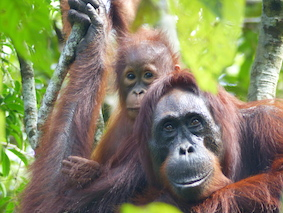
\includegraphics{EigGen/P1030879}}
\begin{quote}
Gestation lasts for 9~months, with females giving birth to their first offspring between the ages of 14 and 15~years. Female orangutans have [seven to] eight-year intervals between births, the longest interbirth intervals among the great apes. \ldots\  Infant orangutans are completely dependent on their mothers for the first two years of their lives. The mother will carry the infant during travelling, as well as feed it and sleep with it in the same night nest. For the first four months, the infant is carried on its belly and never relieves physical contact. In the following months, the time an infant spends with its mother decreases. When an orangutan reaches the age of two, its climbing skills improve and it will travel through the canopy holding hands with other orangutans, a behaviour known as ``buddy travel". Orangutans are juveniles from about two to five years of age and will start to temporarily move away from their mothers.  Juveniles are usually weaned at about four years of age. Adolescent orangutans will socialize with their peers while still having contact with their mothers. Typically, orangutans live over 30~years in both the wild and captivity.
\end{quote}
Suppose the initial population of orangutans in some area at year zero of a study is that of \(30\)~adolescent females and \(15\)~adult females.
Use the mathematical model to predict the population for the next five years.

\begin{solution} 
\emph{Choose level:}  we choose a time unit of one year, and choose to model three age categories.%
\footnote{A coarse model considers just the total number in a species; a fine model might count the number of each age in years (here 30~years); a `micro' model might simulate each and every orangutan as individuals (thousands).}

\emph{Define:}
\begin{itemize}
\item \(y_1(t)\) is the number of \idx{juvenile} \idx{female}s (including infant) at time~\(t\)~(years), say age\({}\leq5\)~years;
\item \(y_2(t)\) is the number of \idx{adolescent} females, say \(6\leq\text{age}\leq 14\)~years;
\item \(y_3(t)\) is the number of \idx{adult} females, say age\({}\geq15\)~years.
\end{itemize}
\emph{Quantify changes in a year:} from Wikipedia information (with numbers slightly modified here to make the results numerically simpler):
\begin{itemize}
\item Orangutans are juvenile for say \(5\)~years, so in any one year a fraction~\(1/5\) of them grow to be adolescent and a fraction~\(4/5\) remain as juveniles.
Say an adult female gives birth every \(7\)--\(8\)~years, so on average it gives birth to a juvenile female every \(15\)~years. 
Thus a fraction~\(1/15\) of adults give birth to a juvenile female in any year.
Consequently, model as \({y_1}(t+1)=\tfrac45y_1(t)+\tfrac1{15}y_3(t)\)\,.
\item Adolescent orangutans become breeding adults after another \(9\)--\(10\)~years, so in any one year a fraction~\(1/10\) of them grow to adults and \(9/10\)ths remain adolescents.
Consequently, \({y_2(t+1)}=+\tfrac15y_1(t)+\tfrac9{10}y_2(t)\)\,.
\item Orangutans live to 30~years, about \(15\)~years of adulthood so in any one year a fraction~\(14/15\) of adult females live to the next year.  
Consequently, \({y_3(t+1)}=\tfrac1{10}y_2(t)+\tfrac9{10}y_3(t)\)\,.
\end{itemize}

The mathematical model of the \idx{age structure} is to let vector \(\yv=(y_1,y_2,y_3)\) then 
\begin{equation*}
\yv(t+1)=A\yv(t)
=\begin{bmatrix} \frac45&0&\frac1{15}
\\\frac15&\frac9{10}&0
\\0&\frac1{10}&\frac{14}{15} \end{bmatrix}\yv(t)
\end{equation*}

To predict the population we need to know the current population.
The given information is that there are initially \(30\)~adolescent females and \(15\)~adult females. 
This information specifies that at time zero the population vector \(\yv(0)=(0,30,15)\) in the study area.
\begin{enumerate}
\item Then the rule \(\yv(t+1)=A\yv(t)\) with time \(t=0\) gives
\begin{eqnarray*}
\yv(1)&=&A\yv(0)
\\&=&\begin{bmatrix} \frac45&0&\frac1{15}
\\\frac15&\frac9{10}&0
\\0&\frac1{10}&\frac{14}{15} \end{bmatrix}\begin{bmatrix} 0\\30\\15 \end{bmatrix}
\\&=&\begin{bmatrix} 1\\27\\17 \end{bmatrix}.
\end{eqnarray*}
That is, during the first year there is one birth of a female juvenile, three adolescents matured to adults, and one adult died. 

\item Then the rule \(\yv(t+1)=A\yv(t)\) with time \(t=1\)~year gives
\begin{eqnarray*}
\yv(2)&=&A\yv(1)
\\&=&\begin{bmatrix} \frac45&0&\frac1{15}
\\\frac15&\frac9{10}&0
\\0&\frac1{10}&\frac{14}{15} \end{bmatrix}\begin{bmatrix} 1\\27\\17 \end{bmatrix}
\\&=&\begin{bmatrix} \frac{29}{15}\\\frac{49}2\\\frac{557}{30} \end{bmatrix}=\begin{bmatrix} 1.93\\24.50\\18.57 \end{bmatrix}\ \twodp.
\end{eqnarray*}
In real life we cannot have such fractions of an orangutan.
These predictions are averages, or expectations on average, and must be interpreted as such. 
Thus after two years, we expect on average nearly two juveniles, \(24\) or~\(25\) adolescents, and \(18\) or~\(19\) adults.

\item Continuing on with the aid of \script\ or calculator, the rule \(\yv(t+1)=A\yv(t)\) with time \(t=2\)~years gives
\begin{eqnarray*}
\yv(3)&=&A\yv(2)
\\&=&\begin{bmatrix} \frac45&0&\frac1{15}
\\\frac15&\frac9{10}&0
\\0&\frac1{10}&\frac{14}{15} \end{bmatrix}
\begin{bmatrix} 1.93\\24.50\\18.57 \end{bmatrix}
\\&=&\begin{bmatrix} 2.78\\22.44\\19.78 \end{bmatrix}\ \twodp.
\end{eqnarray*}
In \script\ do this calculation via
\begin{verbatim}
A=[4/5 0 1/15;1/5 9/10 0;0 1/10 14/15]
y0=[0;30;15]
y1=A*y0
y2=A*y1
y3=A*y2
y4=A*y3
y5=A*y4
\end{verbatim}
\setbox\ajrqrbox\hbox{\qrcode{% orangutans
A=[4/5 0 1/15;1/5 9/10 0;0 1/10 14/15]
y0=[0;30;15]
y1=A*y0
y2=A*y1
y3=A*y2
y4=A*y3
y5=A*y4
}}%
\marginpar{\usebox{\ajrqrbox}}%

\item Consequently, the rule \(\yv(t+1)=A\yv(t)\) with time \(t=3\)~years gives
\begin{eqnarray*}
\yv(4)&=&A\yv(3)
\\&=&\begin{bmatrix} \frac45&0&\frac1{15}
\\\frac15&\frac9{10}&0
\\0&\frac1{10}&\frac{14}{15} \end{bmatrix}
\begin{bmatrix} 2.78\\22.44\\19.78 \end{bmatrix}
\\&=&\begin{bmatrix} 3.55\\20.75\\20.70 \end{bmatrix}\ \twodp.
\end{eqnarray*}
  
\item Lastly, the rule \(\yv(t+1)=A\yv(t)\) with time \(t=4\)~years gives
\begin{eqnarray*}
\yv(5)&=&A\yv(4)
\\&=&\begin{bmatrix} \frac45&0&\frac1{15}
\\\frac15&\frac9{10}&0
\\0&\frac1{10}&\frac{14}{15} \end{bmatrix}
\begin{bmatrix} 3.55\\20.75\\20.70 \end{bmatrix}
\\&=&\begin{bmatrix} 4.22\\19.38\\21.40 \end{bmatrix}\ \twodp.
\end{eqnarray*}
Thus after five years the mathematical model predicts about \(4\)~juveniles, \(19\)~adolescents, and \(21\)~adults (on average).
\marginpar{\begin{tikzpicture}
\def\temp#1{\addplot+ table[x=t,y=y#1,row sep=\\] {
    t       y1     y2      y3 \\
    0.00    0.00   30.00   15.00 \\
    1.00    1.00   27.00   17.00 \\
    2.00    1.93   24.50   18.57 \\
    3.00    2.78   22.44   19.78 \\
    4.00    3.55   20.75   20.70 \\
    5.00    4.22   19.38   21.40 \\
};
\addlegendentry{$y_#1(t)$};
}
\begin{axis}[footnotesize,font=\footnotesize, 
xlabel={$t$\,yrs},ylabel={$y_j$},axis lines=middle
,only marks,xmax=5.4,legend pos=south west]
\temp1
\temp2
\temp3
\end{axis}
\end{tikzpicture}}%
\end{enumerate}
Notice that the five-year population of \(44\)~females (\(45\)~if you add all the fractions) is the same as the starting population.
This nearly static total population is no accident, as we next see, and contributes to why orangutans are critically endangered.
%\emph{Interpret} Two of the three modes decay like~\(e^{-t/5}\) so after ten years or so they are negligible. 
%What emerges is the remaining mode with age structure of  20\%~juveniles, 40\%~adolescents, and 40\%~adults.
%A further prediction is that this population remains constant.
%Although we fudged the numbers somewhat, this implies that orangutan survival is easily damaged by small influences. 
\end{solution}
\end{example}


The mathematical model \(\yv(t+1)=A\yv(t)\) does forecast the future populations.
However, to make predictions for many years and for general initial populations we prefer the formula solution given by the next Theorem~\ref{thm:dynsol} and introduced in the next example.

\begin{example} \label{eg:2x2map}
A vector \(\yv(t)\in\RR^2\) changes with time~\(t\) according to 
\begin{equation*}
\yv(t+1)=A\yv(t)=\begin{bmatrix} 1&-1\\-4&1 \end{bmatrix}\yv(t).
\end{equation*}
First, what is \(\yv(3)\) if the initial \(\yv(0)=(0,1)\)?
Second, find a general formula for~\(\yv(t)\) from any~\(\yv(0)\).
\begin{solution} 
First, given \(\yv(0)=(0,1)\) just compute (as drawn in the margin)
\begin{eqnarray*}
\yv(1)&=&A\yv(0)=\begin{bmatrix} 1&-1\\-4&1 \end{bmatrix}
\begin{bmatrix} 0\\1 \end{bmatrix}
=\begin{bmatrix} -1\\1 \end{bmatrix},
\\\yv(2)&=&A\yv(1)=\begin{bmatrix} 1&-1\\-4&1 \end{bmatrix}
\begin{bmatrix} -1\\1 \end{bmatrix}
=\begin{bmatrix} -2\\5 \end{bmatrix},
\\\yv(3)&=&A\yv(2)=\begin{bmatrix} 1&-1\\-4&1 \end{bmatrix}
\begin{bmatrix} -2\\5 \end{bmatrix}
=\begin{bmatrix} -7\\13 \end{bmatrix}.
\end{eqnarray*}
\marginpar{\begin{tikzpicture}
\begin{axis}[footnotesize,font=\footnotesize,domain=0:3, 
xlabel={time $t$},ylabel={$y_j$},axis lines=middle
,only marks,samples=4,xmax=3.9]
\addplot+ {0.25*(-1)^x-0.25*3^x};
\addlegendentry{$y_1(t)$};
\addplot+ {0.25*(-1)^x*2+0.25*3^x*2};
\addlegendentry{$y_2(t)$};
\end{axis}
\end{tikzpicture}}


Second, let's suppose there may be solutions in the form \(\yv=\lambda^t\vv\) for some non-zero scalar~\(\lambda\) and some vector \(\vv\in\RR^2\).
Substitute into \(\yv(t+1)=A\yv(t)\) to find \(\lambda^{t+1}\vv=A\lambda^t\vv\). 
Divide by (non-zero) \(\lambda^t\) to find we require \(A\vv=\lambda\vv\)\,: this is an \idx{eigen-problem}.
That is, for every eigenvalue~\(\lambda\) with corresponding eigenvector~\vv\ there is a solution \(\yv=\lambda^t\vv\).

To find the eigenvalues here solve the characteristic equation 
\begin{equation*}
\det(A-\lambda I)=\begin{vmatrix} 1-\lambda&-1\\-4&1-\lambda \end{vmatrix}=(1-\lambda)^2-4=0\,.
\end{equation*}
Rearrange to \((\lambda-1)^2=4\) and take square roots to give \(\lambda-1=\pm2\)\,, that is, eigenvalues \(\lambda=1\pm2=-1,3\)\,.
\begin{itemize}
\item For eigenvalue \(\lambda_1=-1\) the corresponding eigenvector has to satisfy
\begin{equation*}
(A+I)\vv_1=\begin{bmatrix} 2&-1\\-4&2 \end{bmatrix}\vv_1=\ov\,.
\end{equation*}
That is, \(\vv_1\propto (1,2)\); let's take \(\vv_1=(1,2)\).

\item For eigenvalue \(\lambda_2=3\) the corresponding eigenvector has to satisfy
\begin{equation*}
(A-3I)\vv_2=\begin{bmatrix} -2&-1\\-4&-2 \end{bmatrix}\vv_2=\ov\,.
\end{equation*}
That is, \(\vv_2\propto (1,-2)\); let's take \(\vv_2=(-1,2)\).
\end{itemize}
Summarising so far: \(\yv'(t)=(-1)^t(1,2)\) and \(\yv''(t)=3^t(-1,2)\) are both solutions of \(\yv(t+1)=A\yv(t)\).

Further, the equation \(\yv(t+1)=A\yv(t)\) is linear in~\yv, so any linear combination of solutions is also a solution.
Let's try \(\yv(t)=c_1\yv'(t)+c_2\yv''(t)\).
Substituting
\begin{eqnarray*}
A\yv(t)&=&A\big(c_1\yv'(t)+c_2\yv''(t)\big)
\\&=&c_1A\yv'(t)+c_2A\yv''(t)
\\&=&c_1\yv'(t+1)+c_2\yv''(t+1)
=\yv(t+1),
\end{eqnarray*}
as required.
So, \(\yv(t)=c_1(-1)^t(1,2)+c_23^t(-1,2)\) are solutions for all constants~\(c_1\) and~\(c_2\), and over all time~\(t\).

Now, what values of constants~\(c_1\) and~\(c_2\) should be chosen for any given initial~\(\yv(0)\)?
Substitute time \(t=0\) into \(\yv(t)=c_1(-1)^t(1,2)+c_23^t(-1,2)\) to require \(\yv(0)=c_1(-1)^0(1,2)+c_23^0(-1,2)\).
Since the zero powers \((-1)^0=3^0=1\)\,, this requires \(\yv(0)=c_1(1,2)+c_2(-1,2)\).
Write as the matrix-vector system
\begin{equation*}
\begin{bmatrix} 1&-1\\2&2 \end{bmatrix}
\begin{bmatrix} c_1\\c_2 \end{bmatrix}
=\yv(0)
\iff
\begin{bmatrix} c_1\\c_2 \end{bmatrix}
=\begin{bmatrix} \frac12&\frac14\\-\frac12&\frac14 \end{bmatrix}\yv(0)
\end{equation*}
upon invoking the inverse (Theorem~\ref{thm:2x2det}) of the matrix of eigenvectors, \(P=\begin{bmatrix} \vv_1&\vv_2 \end{bmatrix}\).
That is, because the matrix of eigenvectors is invertible, we find constants~\(c_1\) and~\(c_2\) to suit any initial~\(\yv(0)\).

For example, with initial \(\yv(0)=(0,1)\) the above formula gives \((c_1,c_2)=(\frac14,\frac14)\) and so the corresponding formula solution is \(\yv(t)=\frac14(-1)^t(1,2)+\frac143^t(-1,2)\).
To check, evaluate at say \(t=3\) to find 
\(\yv(3)=-\frac14(1,2)+\frac{27}4(-1,2)=(-7,13)\),
as before.
In general, as here, as time~\(t\) increases, the solution~\(\yv(t)\) grows like~\(3^t\) with a little oscillation from the~\((-1)^t\) term.
\end{solution}
\end{example}


\begin{theorem} \label{thm:dynsol}
Suppose the \(n\times n\) \idx{square matrix}~\(A\) governs the dynamics of \(\yv(t)\in\RR^n\) according to \(\yv(t+1)=A\yv(t)\).
\begin{enumerate}
\item\label{thm:dynsola} Let \hlist\lambda m\ be \idx{eigenvalue}s of~\(A\) and \hlist\vv m\ be corresponding \idx{eigenvector}s, then a solution of \(\yv(t+1)=A\yv(t)\) is the \idx{linear combination}
\begin{equation}
\yv(t)=c_1\lambda_1^t\vv_1+c_2\lambda_2^t\vv_2+\cdots+c_m\lambda_m^t\vv_m
\label{eq:dynsol}
\end{equation}
for all constants \hlist cm.

\item\label{thm:dynsolb} Further, if the number of eigenvectors \(m=n\), the size of the matrix, and the matrix of eigenvectors \(P=\begin{bmatrix} \vv_1&\vv_2&\cdots&\vv_n \end{bmatrix}\) is \idx{invertible}, then the general linear combination~\eqref{eq:dynsol} is a \bfidx{general solution} in that constants \hlist cn\ can be found for every given initial~\(\yv(0)\).
\end{enumerate}
\end{theorem}

\begin{proof} \ 
\begin{itemize}
\item[\ref{thm:dynsola}] 
Just premultiply~\eqref{eq:dynsol} by matrix~\(A\) to find that
\begin{eqnarray*}
A\yv(t)&=&A(c_1\lambda_1^t\vv_1+c_2\lambda_2^t\vv_2+\cdots+c_m\lambda_m^t\vv_m)
\\&&\quad(\text{using distributivity Thm.~\ref{thm:pasm}})
\\&=&c_1\lambda_1^tA\vv_1+c_2\lambda_2^tA\vv_2+\cdots+c_m\lambda_m^tA\vv_m
\\&&\quad(\text{as eigenvectors }A\vv_j=\lambda_j\vv_j)
\\&=&c_1\lambda_1^t\lambda_1\vv_1+c_2\lambda_2^t\lambda_2\vv_2+\cdots+c_m\lambda_m^t\lambda_m\vv_m
\\&=&c_1\lambda_1^{t+1}\vv_1+c_2\lambda_2^{t+1}\vv_2+\cdots+c_m\lambda_m^{t+1}\vv_m
\end{eqnarray*}
which is the given formula~\eqref{eq:dynsol} for~\(\yv(t+1)\).
Hence \eqref{eq:dynsol} is a solution of \(\yv(t+1)=A\yv(t)\).

\item[\ref{thm:dynsolb}]
For any given initial value~\(\yv(0)\), the solution~\eqref{eq:dynsol} will hold if we can find constants \hlist cm\ such that the solution~\eqref{eq:dynsol} evaluates to~\(\yv(0)\) at time \(t=0\)\,.
Let's do this given the preconditions that the number of eigenvectors \(m=n\) and the matrix \(P=\begin{bmatrix} \vv_1&\vv_2&\cdots&\vv_n \end{bmatrix}\) is {invertible}.
Evaluating the solution~\eqref{eq:dynsol} at \(t=0\) we need to solve, since the zeroth power \(\lambda_j^0=1\)\,,
\begin{equation*}
\yv(0)=\lincomb c\vv n\,.
\end{equation*}
Writing as a matrix-vector system this equation requires \(P\cv=\yv(0)\) for constant vector \(\cv=(\hlist cn)\).
Since \(P\)~is invertible, \(P\cv=\yv(0)\) always has the unique solution \(\cv=P^{-1}\yv(0)\) (Theorem~\ref{thm:ftim2}) which are the requisite constants.
\end{itemize}
\end{proof}




\begin{example} \label{eg:2x2ccgrow}
Consider the dynamics of \(\yv(t+1)=A\yv(t)\) for matrix \(A=\begin{bmatrix} 1&3\\-1&1 \end{bmatrix}\).
First, what is \(\yv(3)\) when the initial~\(\yv(0)=(1,0)\)?
Second, find a \idx{general solution}.
% and interpret its behaviour in time~\(t\).
\begin{solution} 
First, just compute (as illustrated)
\begin{eqnarray*}
\yv(1)&=&A\yv(0)=\begin{bmatrix} 1&3\\-1&1 \end{bmatrix}
\begin{bmatrix} 1\\0 \end{bmatrix}
=\begin{bmatrix} 1\\-1 \end{bmatrix},
\\\yv(2)&=&A\yv(1)=\begin{bmatrix} 1&3\\-1&1 \end{bmatrix}
\begin{bmatrix} 1\\-1 \end{bmatrix}
=\begin{bmatrix} -2\\-2 \end{bmatrix},
\\\yv(3)&=&A\yv(2)=\begin{bmatrix} 1&3\\-1&1 \end{bmatrix}
\begin{bmatrix} -2\\-2 \end{bmatrix}
=\begin{bmatrix} -8\\0 \end{bmatrix}.
\end{eqnarray*}
\marginpar{\begin{tikzpicture}
\begin{axis}[footnotesize,font=\footnotesize, 
xlabel={time $t$},ylabel={$y_j$},axis lines=middle
,only marks,xmax=3.9,legend pos=south west]
\addplot+ coordinates {(0,1)(1,1)(2,-2)(3,-8)};
\addlegendentry{$y_1(t)$};
\addplot+ coordinates {(0,0)(1,-1)(2,-2)(3,0)};
\addlegendentry{$y_2(t)$};
\end{axis}
\end{tikzpicture}}%
Interestingly, after three steps in time~\(\yv(3)\) is~\((-8)\) times the initial~\(\yv(0)\).
This suggest after six steps in time \(\yv(6)\) will be \((-8)^2=64\) times the initial~\(\yv(0)\), and so on.
Perhaps the solution grows in size roughly like~\(2^t\) but in some irregular manner.

Second, find a general solution via the eigenvalues and eigenvectors of the matrix~\(A\).  
Its characteristic equation is 
\begin{equation*}
\det(A-\lambda I)=\begin{vmatrix} 1-\lambda&3\\-1&1-\lambda \end{vmatrix}
=(1-\lambda)^2+3=0\,.
\end{equation*}
That is, \((\lambda-1)^2=-3\) which upon taking square roots gives the complex conjugate pair of eigenvalues \(\lambda=1\pm i\sqrt3\).
Theorem~\ref{thm:dynsol} applies for \idx{complex eigenvalue}s and eigenvectors so we proceed.
\begin{itemize}
\item For eigenvalue \(\lambda_1=1+i\sqrt3\) the corresponding eigenvectors~\(\vv_1\) satisfy
\begin{equation*}
(A-(1+i\sqrt3)I)\vv_1=\begin{bmatrix} -i\sqrt3&3\\-1&-i\sqrt3 \end{bmatrix}\vv_1=\ov\,.
\end{equation*}
Solutions are proportional to \(\vv_1=(-i\sqrt3,1)\).

\item For eigenvalue \(\lambda_2=1-i\sqrt3\) the corresponding eigenvectors~\(\vv_2\) satisfy
\begin{equation*}
(A-(1-i\sqrt3)I)\vv_2=\begin{bmatrix} i\sqrt3&3\\-1&i\sqrt3 \end{bmatrix}\vv_2=\ov\,.
\end{equation*}
Solutions are proportional to \(\vv_2=(+i\sqrt3,1)\).
\end{itemize}
Theorem~\ref{thm:dynsol} then establishes that a solution to \(\yv(t+1)=A\yv(t)\) is
\begin{equation*}
\yv(t)=c_1(1+i\sqrt3)^t\begin{bmatrix} -i\sqrt3\\1 \end{bmatrix}
+c_2(1-i\sqrt3)^t\begin{bmatrix} +i\sqrt3\\1 \end{bmatrix}.
\end{equation*}
This is a general solution since the matrix of the two eigenvectors (albeit complex valued) is invertible:
\begin{equation*}
P=\begin{bmatrix} \vv_1&\vv_2 \end{bmatrix}
=\begin{bmatrix} -i\sqrt3&i\sqrt3\\1&1 \end{bmatrix}
\quad\text{has }
P^{-1}=\begin{bmatrix} \frac i{2\sqrt3}&\frac12\\\frac{-i}{2\sqrt3}&\frac12 \end{bmatrix}
\end{equation*}
as its inverse (Theorem~\ref{thm:2x2det}).

For example, if \(\yv(0)=(1,0)\), then the coefficient constants are \((c_1,c_2)=P^{-1}(1,0)=(i,-i)/(2\sqrt3)\).
Then the solution becomes
\begin{eqnarray*}
\yv(t)&=&\frac i{2\sqrt3}(1+i\sqrt3)^t\begin{bmatrix} -i\sqrt3\\1 \end{bmatrix}
-\frac{i}{2\sqrt3}(1-i\sqrt3)^t\begin{bmatrix} +i\sqrt3\\1 \end{bmatrix}
\\&=&\tfrac 12(1+i\sqrt3)^t\begin{bmatrix} 1\\\frac i{\sqrt3} \end{bmatrix}
+\tfrac12(1-i\sqrt3)^t\begin{bmatrix} 1\\-\frac i{\sqrt3} \end{bmatrix}.
\end{eqnarray*}
Through the magic of the complex conjugate form of the two terms in this expression, the complex parts cancel to always give a real result.
For example, this complex formula predicts at time step \(t=1\)
\begin{eqnarray*}
\yv(1)&=&\tfrac 12(1+i\sqrt3)\begin{bmatrix} 1\\\frac i{\sqrt3} \end{bmatrix}
+\tfrac12(1-i\sqrt3)\begin{bmatrix} 1\\-\frac i{\sqrt3} \end{bmatrix}
\\&=&\frac12\begin{bmatrix} 1+i\sqrt3+1-i\sqrt3\\
\frac i{\sqrt3}-1-\frac i{\sqrt3}-1 \end{bmatrix}
\\&=&\begin{bmatrix} 1\\-1 \end{bmatrix},
\end{eqnarray*}
as computed directly at the start of this example.
\end{solution}
\end{example}

One crucial qualitative aspect we need to know is whether components in the solution~\eqref{eq:dynsol} grow, decay, or stay the same size as time increases.
This is determined by the eigenvalues as~\(\lambda_j^t\) is the only place that the time appears in the formula~\eqref{eq:dynsol}.
\begin{itemize}
\item For example, in the general solution for Example~\ref{eg:2x2map}, \(\yv(t)=c_1(-1)^t(1,2)+c_23^t(-1,2)\), the \(3^t\)~factor grows in time since \(3^1=3\), \(3^2=9\), \(3^3=27\), and so on.
Whereas the \((-1)^t\)~factor just oscillates in time since \((-1)^1=-1\), \((-1)^2=1\), \((-1)^3=-1\), and so on.
Thus for long times we know that the term involving the factor~\(3^t\) will dominate the solution as it grows.

\item In Example~\ref{eg:2x2ccgrow} with complex conjugate eigenvalues the situation is more complicated.
Let's write any given \idx{complex eigenvalue} in \idx{polar form} 
\(\lambda=r(\cos\theta+i\sin\theta)\) where magnitude \(r=|\lambda|\) and angle~\(\theta\) such that \(\tan\theta=(\Im\lambda)/(\Re\lambda)\).
For example, \(1-i\) has magnitude \(r=|1-1i|=\sqrt{1^2+(-1)^2}=\sqrt2\) and angle \(\theta=-\frac\pi4\) since \(\tan(-\frac\pi4)=-1/1\)\,.
Question: how does this help understand the solution which has \(\lambda_j^t\) in it?
Answer: \idx{De Moivre's theorem} says that if \(\lambda=r[\cos\theta+i\sin\theta]\), then \(\lambda^t=r^t\big[\cos(\theta t)+i\sin(\theta t)\big]\).
Since the magnitude \(|\cos(\theta t)+i\sin(\theta t)|=\sqrt{\cos^2(\theta t)+\sin^2(\theta t)}=\sqrt1=1\)\,, the magnitude \(|\lambda^t|=r^t\).
For example, the magnitude \(|(1-i)^2|=(\sqrt2)^2=2\) which we check by computing \((1-i)^2=1^2-2i+i^2=-2i\) and \(|-2i|=2\)\,.

In Example~\ref{eg:2x2ccgrow}, the eigenvalue \(\lambda_1=1+i\sqrt3\) so its magnitude is \(r_1=|\lambda_1|=|1+i\sqrt3|=\sqrt{1+3}=2\)\,.
%Its angle \(\theta_1=\frac\pi3\) because \(\tan\frac\pi3=\sqrt3=\sqrt3/1\)\,.
Hence the magnitude \(|\lambda_1^t|=2^t\) at any time step~\(t\).
Similarly, the magnitude \(|\lambda_2^t|=2^t\) at any time step~\(t\).
Consequently, the general solution
\begin{equation*}
\yv(t)=c_1\lambda_1^t\begin{bmatrix} -i\sqrt3\\1 \end{bmatrix}
+c_2\lambda_2^t\begin{bmatrix} +i\sqrt3\\1 \end{bmatrix}
\end{equation*}
will grow in magnitude roughly like~\(2^t\) as both components grow like~\(2^t\).
It is a `rough' growth because the components \(\cos(\theta t)\) and~\(\sin(\theta t)\)  cause `oscillations' in time~\(t\).
Nonetheless the overall growth like \(|\lambda_1|^t=|\lambda_2|^t=2^t\) is inexorable---and seen previously in the particular solution where we observe \(\yv(3)\) is eight times the magnitude of~\(\yv(0)\).
\end{itemize}
In general, for both real or complex eigenvalues~\(\lambda\), a term involving the factor~\(\lambda^t\) will, as time~\(t\) increases,
\marginpar{\begin{tikzpicture}
\begin{axis}[footnotesize,font=\footnotesize,domain=0:10, 
xlabel={time $t$},ylabel={$|\lambda|^t$},axis lines=middle
,only marks,samples=11,ymin=0,xmax=11.5]
\addplot+ {1.16^x};
\addlegendentry{$|\lambda|>1$};
\addplot+ {0.8^x};
\addlegendentry{$|\lambda|<1$};
\addplot+ {1^x};
\addlegendentry{$|\lambda|=1$};
\end{axis}
\end{tikzpicture}}
\begin{itemize}
\item grow to infinity if \(|\lambda|>1\)\,,
\item decay to zero if \(|\lambda|<1\)\,, and
\item remain the same magnitude if \(|\lambda|=1\)\,.
\end{itemize}





\begin{example}[orangutans over many years] \label{eg:orangs}
Extend orangutan analysis of Example~\ref{eg:orang}. 
Use Theorem~\ref{thm:dynsol} to predict the population over many years: from an initial population of \(30\)~adolescent females and \(15\)~adult females; and from a general initial population.
\begin{solution} 
Example~\ref{eg:orang} derived that the age structure population \(\yv=(y_1,y_2,y_3)\) satisfies \(\yv(t+1)=A\yv(t)\) for matrix
\begin{equation*}
A=\begin{bmatrix} \frac45&0&\frac1{15}
\\\frac15&\frac9{10}&0
\\0&\frac1{10}&\frac{14}{15} \end{bmatrix}.
\end{equation*}
Let's find the eigenvalues and eigenvectors of the matrix~\(A\) using \script\ via
\begin{verbatim}
A=[4/5 0 1/15;1/5 9/10 0;0 1/10 14/15]
[V,D]=eig(A)
\end{verbatim}
\setbox\ajrqrbox\hbox{\qrcode{% orangutans
A=[4/5 0 1/15;1/5 9/10 0;0 1/10 14/15]
[V,D]=eig(A)
y0=[0;30;15]
rcond(V)
c=V\slosh y0
}}%
\marginpar{\usebox{\ajrqrbox}}%
to find
\begin{verbatim}
V =
 -0.3077+0.2952i -0.3077-0.2952i  0.2673+0.0000i
  0.7385+0.0000i  0.7385+0.0000i  0.5345+0.0000i
 -0.4308-0.2952i -0.4308+0.2952i  0.8018+0.0000i
D =
  0.8167+0.0799i  0.0000+0.0000i  0.0000+0.0000i
  0.0000+0.0000i  0.8167-0.0799i  0.0000+0.0000i
  0.0000+0.0000i  0.0000+0.0000i  1.0000+0.0000i
\end{verbatim}
Evidently there is one real eigenvalue of \(\lambda_3=1\) and two complex conjugate eigenvalues \(\lambda_{1,2}=0.8167\pm i0.0799\)\,.
Corresponding eigenvectors are the columns~\(\vv_j\) of~\(V\).
Thus a solution for the orangutan population is
\begin{equation*}
\yv(t)=c_1\lambda_1^t\vv_1+c_2\lambda_2^t\vv_2+c_3\lambda_3^t\vv_3\,.
\end{equation*}
\begin{itemize}
\item For the initial population \(\yv(0)=(0,30,15)\) we need to find constants \(\cv=(c_1,c_2,c_3)\) such that \(V\cv=\yv(0)\).
Solve this linear equation in \script\ with 
\begin{verbatim}
y0=[0;30;15]
rcond(V)
c=V\y0
\end{verbatim}
which gives the answer
\begin{verbatim}
ans =
    0.1963
c =
  10.1550+2.1175i
  10.1550-2.1175i
  28.0624+0.0000i
\end{verbatim}
The \verb|rcond| value of~\(0.1963\) indicates that matrix~\(V\) is invertible.
Then the backslash operator computes the above coefficients~\cv.
Via the magic of complex conjugates cancelling, the real population of orangutans is for all times predicted to be \twodp
\begin{eqnarray*}
\yv(t)&=&(10.16+2.12i)(0.82+0.08i)^t\begin{bmatrix} -0.31+0.30i   \\0.74
\\-0.43-0.30i \end{bmatrix}
\\&&{}
+(10.16-2.12i)(0.82+0.08i)^t\begin{bmatrix} -0.31-0.30i   \\0.74
\\-0.43+0.30i \end{bmatrix}
\\&&{}
+28.06\begin{bmatrix} 0.27
\\0.53
\\0.80 \end{bmatrix}
\end{eqnarray*}
since \(\lambda_3^t=1^t=1\)\,.

Since the magnitude \(|\lambda_1|=|\lambda_2|=0.82\) \twodp, 
the first two terms in this expression decay to zero as time~\(t\) increases.
For example, \(|\lambda_1^{12}|=|\lambda_2^{12}|=0.09\)\,.
Hence the model predicts that over long times the population
\begin{equation*}
\yv(t)\approx 28.06\begin{bmatrix} 0.27
\\0.53
\\0.80 \end{bmatrix}
=\begin{bmatrix} 7.5\\15.0\\22.5 \end{bmatrix}
\end{equation*}
Such a static population means that the orangutans are highly sensitive to disease, or deforestation, or chance events, and so on.

\item Such unfortunate sensitivity is typical for orangutans.  
It is not a quirk of the initial population.
Recall the general prediction for the orangutans is 
\begin{equation*}
\yv(t)=c_1\lambda_1^t\vv_1+c_2\lambda_2^t\vv_2+c_3\lambda_3^t\vv_3\,.
\end{equation*}
The initial population determines the constants~\(\cv\).
However, the long term population is always predicted to be static.
The reason is that the magnitude of the eigenvalues \(|\lambda_1|=|\lambda_2|=0.82\) and so the first two terms in this general solution will in time always decay to zero.
Further, the remaining third eigenvalue has magnitude \(|\lambda_3|=|1|=1\) and so the third term in the population prediction is always constant in time~\(t\).
That is, over long times the population is always
\begin{equation*}
\yv(t)\approx c_3\vv_3\,.
\end{equation*}
Such a static population means that the orangutans are always sensitive to  disease, or deforestation, or chance events, and so on.

\end{itemize}
\end{solution}
\end{example}




\cite{gaimme2016} discuss mathematical modelling.
On page~23 they comment ``\emph{Modelling (like real life) is open-ended and messy}'': in our two examples here you have to extract the important factors from many unneeded details, and use them in the context of an imperfect model.
\cite{gaimme2016} [p.23] also comment that modellers ``\emph{must be making genuine choices}'': in these problems, as in all modelling, there are choices that lead to different models---we have to operate and sensibly predict with such uncertainty.
Lastly, \cite{gaimme2016} recommend to ``\emph{focus on the process, not the product}'': depending upon your choices and interpretations you will develop alternative plausible models in these scenarios---it is the process of forming plausible models and interpreting the results that are important here.



\begin{example}[servals grow] \label{eg:serval} 
The \idx{serval} is a member of the cat family that lives in Africa.
Given next is an extract from \idx{Wikipedia} of a serval's Reproduction and Life History.
\marginpar{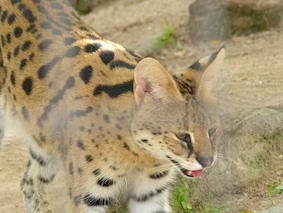
\includegraphics{EigGen/P1040280}}
\begin{quote}
Kittens are born shortly before the peak breeding period of local rodent populations. A serval is able to give birth to multiple litters throughout the year, but commonly does so only if the earlier litters die shortly after birth. Gestation lasts from~66 to 77~days and commonly results in the birth of two kittens, although sometimes as few as one or as many as four have been recorded.

The kittens are born in dense vegetation or sheltered locations such as abandoned aardvark burrows. If such an ideal location is not available, a place beneath a shrub may be sufficient. The kittens weigh around~250\,gm at birth, and are initially blind and helpless, with a coat of greyish woolly hair. They open their eyes at~9 to 13~days of age, and begin to take solid food after around a month. At around six months, they acquire their permanent canine teeth and begin to hunt for themselves; they leave their mother at about 12~months of age. They may reach sexual maturity from~12 to 25~months of age.

Life expectancy is about 10~years in the wild.
\end{quote}
From the information in this extract, create a plausible, \idx{age structure}d,  \idx{population model} of the \idx{serval}: give reasons for estimates of the coefficients in the model.
Choose three age categories of \idx{kitten}s, \idx{juvenile}s, sexually mature \idx{adult}s.
What does the model predict over long times?
\begin{solution} 
Recall we only model the number of \emph{female} servals as females are the limiting breeders.
Define 
\begin{itemize}
\item \(y_1(t)\) is the number of female kittens, less than 0.5~years old from when they ``begin to hunt for themselves'';
\item \(y_2(t)\) is the number of female juveniles, between 0.5~years and 1.5~years which is when they ``reach sexual maturity'' on average;
\item \(y_3(t)\) is the number of female breeding adults, older than 1.5~years, and dying at about the ``life expectancy'' of 10~years;
\item since servals transition from one age category to another in multiples of six months (0.5~years), let the unit of time be six~months, equivalently a half-year.  
Consequently, time~\(t+1\) is the time a half-year later than time~\(t\).
\end{itemize}
Modelling of the servals leads to the following equations.
\begin{itemize}
\item Kittens are commonly born once a year to each female, and the common litter size is two, so \emph{on average} one female kitten is born per year per adult, that is, on average \(\frac12\)~female kitten is born per half-year per adult female:
Also all kittens age to juveniles after 0.5~years, so none remain as kittens.  
Hence the kitten equation is \(y_1(t+1)=0y_1(t)+\tfrac12y_3(t)\).
\item Juveniles mature from the kittens, and age to an adult after about one year: that is, on average half of them become adults every half-year, and half remain juveniles.
So the juvenile equation is \(y_2(t+1)=y_1(t)+\tfrac12y_2(t)\).
\item Adults mature from the juveniles, and die after about 8.5~years which is about a rate \(1/8.5\)~per year: that is, a rate of \(\frac1{17}\)~per half-year leaving \(\tfrac{16}{17}\) of them to live into the next half-year.
So the adult equation is \( y_3(t+1)=\tfrac12y_2(t)+\tfrac{16}{17}y_3(t)\).
\end{itemize}

Bring these equations together, the age structure population \(\yv=(y_1,y_2,y_3)\) satisfies \(\yv(t+1)=A\yv(t)\) for matrix
\begin{equation*}
A=\begin{bmatrix} 0&0&\frac1{2}
\\1&\frac12&0
\\0&\frac12&\frac{16}{17} \end{bmatrix}.
\end{equation*}
Find the eigenvalues and eigenvectors of the matrix~\(A\) using \script\ via
\begin{verbatim}
A=[0 0 1/2;1 1/2 0;0 1/2 16/17]
[V,D]=eig(A)
\end{verbatim}
\setbox\ajrqrbox\hbox{\qrcode{% servals
A=[0 0 1/2;1 1/2 0;0 1/2 16/17]
[V,D]=eig(A)
}}%
\marginpar{\usebox{\ajrqrbox}}%
to find
\begin{verbatim}
V =
 -0.3066+0.3439i -0.3066-0.3439i  0.3352+0.0000i
  0.7838+0.0000i  0.7838+0.0000i  0.4633+0.0000i
 -0.3684-0.1942i -0.3684+0.1942i  0.8203+0.0000i
D =
  0.1088+0.4387i  0.0000+0.0000i  0.0000+0.0000i
  0.0000+0.0000i  0.1088-0.4387i  0.0000+0.0000i
  0.0000+0.0000i  0.0000+0.0000i  1.2236+0.0000i
\end{verbatim}
Evidently there is one real eigenvalue of \(\lambda_3=1.2236\) and two complex conjugate eigenvalues \(\lambda_{1,2}=0.1088\pm i0.4387\)\,.
Corresponding eigenvectors are the columns~\(\vv_j\) of~\(V\).
Thus a general solution for the serval population is (Theorem~\ref{thm:dynsol})
\begin{equation*}
\yv(t)=c_1\lambda_1^t\vv_1+c_2\lambda_2^t\vv_2+c_3\lambda_3^t\vv_3\,.
\end{equation*}

In this general solution, the first two terms will decay in time to zero.
The reason is that the magnitudes \(|\lambda_1|=|\lambda_2|=|0.1088\pm i0.4387|=\sqrt{0.1088^2+0.4387^2}=0.4520\), and since this magnitude is less than one, then \(\lambda_1^t\) and~\(\lambda_2^t\) will decay to zero with increasing time~\(t\).
However, the third term increases in time as \(\lambda_3=1.2236>1\)\,.
The model predicts the serval population increases by about~22\% per half-year (about~50\% per year).
\end{solution} 
Predation, disease, and food shortages are just some processes not included in this model which act to limit the serval's population in ways not included in this model.
\end{example}





Crucial in this section---so that we find a solution for all initial states---is that the matrix of eigenvectors is invertible.
The next Section~\ref{sec:lisb} relates the invertibility of a matrix of eigenvectors to the concept of `linear independence' defined in that section (Theorem~\ref{thm:ftim3}).



\index{age structure|)}
\index{population|)}





%\begin{comment}
%\subsection{Metastability in Markov chains}
%Ensure application-like.
%\end{comment}








\subsection{Extension: Connect SVDs to eigen-problems}

Recall that Chapter~\ref{ch:eesm} starts by illustrating the close connection between the \svd\ of a symmetric matrix and the eigenvalues and eigenvectors of that symmetric matrix.
\begin{aside}
This optional section connects the \svd\ of a general matrix to a symmetric eigen-problem, in principle.
\end{aside}%
This subsection establishes that an \svd\ of a general matrix is closely connected to the eigenvalues and eigenvectors of a specific matrix of double the size.   
The connection depends upon determinants and solving linear systems and so, in principle, is an approach to compute an \svd\ distinct from the inductive maximisation.



\begin{example} \label{eg:eigsvd}
Compute the eigenvalues and eigenvectors of the (symmetric) matrix
\begin{equation*}
B=\begin{bmatrix} 0&0&10&2\\
0&0&5&11\\
10&5&0&0\\
2&11&0&0 \end{bmatrix}.
\end{equation*}
\begin{solution} In \script\ execute
\setbox\ajrqrbox\hbox{\qrcode{% eigenvalue/vector code
B=[0 0 10 2
   0 0 5 11
  10 5 0 0
  2 11 0 0]
[V,D]=eig(B)
}}%
\marginpar{\usebox{\ajrqrbox}}%
\begin{verbatim}
B=[0 0 10 2
   0 0 5 11
  10 5 0 0
  2 11 0 0]
[V,D]=eig(B)
\end{verbatim}
and obtain \twodp
\begin{verbatim}
V =
   0.42   0.57   0.57  -0.42
   0.57  -0.42  -0.42  -0.57
  -0.50  -0.50   0.50  -0.50
  -0.50   0.50  -0.50  -0.50
D =
  -14.14       0       0       0
       0   -7.07       0       0
       0       0    7.07       0
       0       0       0   14.14
\end{verbatim}
The eigenvalues are the pairs \(\pm7.07\) and \(\pm14.14\), with corresponding eigenvector pairs \((0.57,-0.42,\pm0.50,\mp0.50)\) and \((\mp0.42,\mp0.57,-0.50,-0.50)\).
\end{solution}
These eigenvalues\slash vectors occur in \(\pm\)~pairs because this matrix has the form
\begin{equation*}
B=\begin{bmatrix} O_2& A\\ \tr A&O_2\end{bmatrix},
\quad\text{here for matrix }
A=\begin{bmatrix} 10&2\\5&11 \end{bmatrix}
\end{equation*}
from Example~\ref{eg:2by2svd}.
Observe that not only are the eigenvectors are orthogonal, because \(B\)~is symmetric, but also the two parts of the eigenvectors are orthogonal:  \((0.57,-0.42)\) from the first pair is orthogonal to \((-0.42,-0.57)\) from the second pair; and \((0.50,-0.50)\) from the first pair is orthogonal to \((-0.50,-0.50)\) from the second pair.
The next Theorem~\ref{thm:eigsvd} establishes how these properties relate to an \svd\ for the matrix~\(A\).
\end{example}


Procedure~\ref{pro:geneig} computes eigenvalues and eigenvectors by hand (in principle no matter how large the matrix). 
The procedure is independent of the \svd.
We now invoke this procedure to find another method to find an \svd\ distinct from the inductive maximisation of the proof in Section~\ref{sec:psvdt}. 
The following theorem is a step towards an efficient numerical computation of an \svd\ \cite[p.234]{Trefethen1997}.

% Trefethen has the transpose in the upper right---curses??


\begin{theorem}[\svd\ as an eigenproblem] \label{thm:eigsvd}
\index{singular value decomposition}\index{SVD}%??
Given an \(m\times n\) matrix~\(A\), the \idx{singular value}s of~\(A\) are the non-negative \idx{eigenvalue}s of the \((m+n)\times(m+n)\) matrix \(B=\begin{bmatrix} O_m&A\\\tr A&O_n \end{bmatrix}\). 
A corresponding \idx{eigenvector}~\(\wv\in\RR^{m+n}\)\ of~\(B\) gives corresponding  singular vectors\index{singular vector} of~\(A\), namely \(\wv=(\uv,\vv)\) for singular vectors \(\uv\in\RR^m\)\ and \(\vv\in\RR^n\). 
\end{theorem}

\begin{proof} 
First prove the \svd\ of~\(A\) gives eigenvalues\slash vectors of~\(B\), and second the converse.
For simplicity this proof considers only the case \(m=n\); the case \(m\neq n\) is similar but the more intricate details are of little interest.

First, let \(n\times n\) matrix \(A=\usv\) be an \svd\ (Theorem~\ref{thm:svd}) for \(n\times n\) orthogonal \(U=\begin{bmatrix} \uv_1&\uv_2&\cdots&\uv_n \end{bmatrix}\),  orthogonal \(V=\begin{bmatrix} \vv_1&\vv_2&\cdots&\vv_n \end{bmatrix}\), and diagonal \(S=\diag(\hlist\sigma n)\).
Post-multiply the \svd\ by orthogonal~\(V\) gives \(AV=US\)\,.
% that is, \(A\vv_j=\sigma_j\uv_j\) for \(j=1,\ldots,n\)\,.
Also, transpose the \svd\ to give \(\tr A=\tr{(\usv)}=V\tr S\tr U=VS\tr U\) and post-multiply by orthogonal~\(U\) to give \(\tr AU=VS\)\,.
% that is, \(\tr A\uv_j=\sigma_j\vv_j\) for \(j=1,\ldots,n\)\,.
Now consider each of the \(\pm\)~cases of
\begin{equation*}
B\begin{bmatrix} U\\\pm V \end{bmatrix}
=\begin{bmatrix} O_n&A\\\tr A&O_n \end{bmatrix}\begin{bmatrix} U\\\pm V \end{bmatrix}
=\begin{bmatrix} \pm AV\\\tr AU \end{bmatrix}
=\begin{bmatrix} \pm US\\VS \end{bmatrix}
=\begin{bmatrix} U\\\pm V \end{bmatrix}(\pm S).
\end{equation*}
Letting \(\wv=(\uv_j,\pm\vv_j)\neq\ov\)\,, the \(j\)th~column of the above equation is \(B\wv=\pm\sigma_j\wv\) and hence \((\uv_j,\pm\vv_j)\) is an eigenvector of~\(B\) corresponding to eigenvalue~\(\pm\sigma_j\), respectively, for \(j=1,\ldots,n\) and each of the \(\pm\)~cases.

Second, let \(\wv\in\RR^{2n}\)\ be an eigenvector of~\(B\) corresponding to an eigenvalue~\(\lambda\) (real as \(B\)~is symmetric, Theorem~\ref{thm:realeigsym}) and normalised so that \(|\wv|=1\)\,.
Partition \(\wv=(\uv,\vv)\) for \(\uv,\vv\in\RR^n\).
Then the fundamental eigen-problem \(B\wv=\lambda\wv\)  (Definition~\ref{def:evecval}) partitions into
\begin{equation}
\begin{bmatrix} O& A\\\tr A&O \end{bmatrix}\begin{bmatrix} \uv\\\vv \end{bmatrix}=\lambda\begin{bmatrix} \uv\\\vv \end{bmatrix}
\iff  A\vv=\lambda\uv \text{ and }\tr A\uv=\lambda\vv\,.
\label{eq:eigsvd}
\end{equation}
Now eigenvalues and eigenvectors of~\(B\) come in pairs as  the eigenvalue \(\lambda'=-\lambda\) corresponds to eigenvector \(\wv'=(\uv,-\vv)\): substitute into~\eqref{eq:eigsvd} to check, \(A(-\vv)=-A\vv=-\lambda\uv=\lambda'\uv\) and \(\tr A\uv=\lambda\vv=(-\lambda)(-\vv)=\lambda'(-\vv)\).
If the eigenvalue~\(\lambda\neq0\)\,, then corresponding to the distinct eigenvalues~\(\pm\lambda\) the eigenvectors \((\uv,\pm\vv)\) of symmetric~\(B\) are orthogonal (Theorem~\ref{thm:orthoevec}) and so \(0=(\uv,\vv)\cdot(\uv,-\vv)=\uv\cdot\uv-\vv\cdot\vv=|\uv|^2-|\vv|^2\) and hence \(|\uv|=|\vv|=\frac1{\sqrt2}\) as \(|\wv|^2=|\uv|^2+|\vv|^2=1\) (see Example~\ref{eg:eigsvd}).
Further, for any two distinct eigenvalues \(|\lambda_i|\neq|\lambda_j|\neq 0\), the eigenvectors \((\uv_i,\vv_i)\) and \((\uv_j,\pm\uv_j)\) are also orthogonal, hence \(0 =(\uv_i,\vv_i)\cdot(\uv_j,\pm\uv_j) =\uv_i\cdot\uv_j \pm\vv_i\cdot\vv_j\)\,.
Taking the sum and the difference of the \(\pm\)~cases of this equation gives \(\uv_i\cdot\uv_j=\vv_i\cdot\vv_j=0\)\,; that is,  (Definition~\ref{def:orthoset}) \(\{\hlist\uv n\}\) and \(\{\hlist\vv n\}\) are both orthogonal sets.
In the cases when matrix~\(B\) has \(2n\)~distinct non-zero eigenvalues, choose \((\uv_j,\vv_j)\) to be a normalised eigenvector corresponding to positive eigenvalue~\(\lambda_j\), \(j=1,\ldots,n\)\,. 
Upon setting \(U=\sqrt2\begin{bmatrix} \uv_1&\uv_2&\cdots&\uv_n \end{bmatrix}\), \(V=\sqrt2\begin{bmatrix} \vv_1&\vv_2&\cdots&\vv_n \end{bmatrix}\), and \(S=\diag(\hlist\lambda n)\), equation~\eqref{eq:eigsvd} gives the columns of \(AV=US\) which since the columns of \(U\) and~\(V\) are orthonormal gives the \svd\ \(A=\usv\) for singular vectors \(\uv_j,\vv_j\in\RR^n\) and singular values~\(\lambda_j(>0)\).

Extensions of this proof cater for the case when zero is an eigenvalue and/or eigenvalues are repeated and/or the dimensions \(m\neq n\)\,.
\end{proof}










\begin{draft}%%%%%%%%%%%%%%%%%%%%%%%
\subsection{Extension: Exponential interpolation discovers dynamics}
\label{sec:eidd}

\index{exponential interpolation|(}

Many applications require identification of rates and frequencies:
\begin{aside}
This optional subsection develops a method useful in some application areas.
\end{aside}%
as a played musical note decays, what is its frequency?
in the observed vibrations of a complicated bridge, what are its natural modes?
in measurements of complicated bio-chemical reactions, what rates can be identified?
All such tasks require fitting a sum of exponential functions to the data.


\begin{example} \label{eg:}
This example is the simplest case of fitting one exponential to two data points.
Suppose we take two measurements of some process: 
\begin{itemize}
\item at time \(t_1=1\) we measure the value \(f_1=5\)\,, and 
\item at time \(t_2=3\) we measure the value \(f_2=10\)\,.
\end{itemize}
Find an exponential fit to this data of the form \(f(t)=ce^{rt}\) for some as yet unknown coefficients~\(c\) and rate~\(r\).
\begin{solution} 
The classic solution is to take logarithms of both sides:
\begin{equation*}
f=ce^{rt} \iff (\ln f)=(\ln c)+rt\,,
\end{equation*}
and then determine \(\ln c\) and~\(r\) by fitting a straight line through the two data points \((t,\ln f)=(1,\ln5)\) and~\((3,\ln10)\)
(recall that \index{ln@\(\ln\)}``\(\ln(x)\)'' denotes the \idx{natural logarithm} of~\(x\),  computed in \script\ with \verb|log(x)|, see Table~\ref{tbl:mtlbmops}).
This approach has the great virtue that the approach generalises to fitting of noisy data (Section~\ref{sec:asie}).
But here we take a different approach that instead generalises to fitting multiple exponentials to more data.

The following simple steps correspond to complicated steps in the general procedure developed next for fitting multiple exponentials.
\begin{enumerate}
\item First, write down the equations that have to be satisfied:
\begin{equation*}
ce^{r}=5\,,\quad ce^{r3}=10\,.
\end{equation*}
\item Second, recognise that the second equation involves the left-hand side of the first:
\begin{equation*}
ce^{r3}=10 \iff ce^re^{r2}=10\iff ce^r\lambda=10
\end{equation*}
for some as yet unknown multiplier \(\lambda=e^{2r}\).
But when we find the multiplier~\(\lambda\), then the rate \(r=\tfrac12\ln\lambda\).
\item Third, eliminate the common part involving the constant~\(c\): since the first equation says \(ce^r=5\), the second equation becomes \(5\lambda=10\)\,.
\item Fourth, no corresponding step here.
\item Fifth, hence the multiplier \(\lambda=2\)\,, giving rate \(r=\tfrac12\ln 2=0.3466\)\,.
\item Finally, determine the constant~\(c\) from, say, \(ce^r=5\)\,:
here \(e^r=\sqrt2\) so \(c=5/\sqrt2=3.5255\)\,.
\end{enumerate}
That is, the exponential fit is \(f(t)=3.5255\,e^{0.3466\,t}\).
\end{solution}
\end{example}







\begin{example} \label{eg:2expfit}
\newcommand{\mytemp}[1]{\begin{tikzpicture}
\begin{axis}[footnotesize,font=\footnotesize
, xlabel={$t$},ylabel={$f$},axis lines=middle
,ymin=0,ymax=1.3,xmax=3.99 ]
\addplot+[mark=*,only marks] coordinates { (0,1) (1,1) (2,2/3) (3,7/18)};
\ifnum1=#1\addplot+[thick,no marks,domain=0:3.99] {-3/3^x+4/2^x};\fi
\end{axis}
\end{tikzpicture}}
Suppose in some chemical or biochemical experiment you measure the concentration of a key chemical at four times (as illustrated): 
\marginpar{\mytemp0}%
at the start of the experiment, time \(t_1=0\) you measure concentration \(f_1=1\) (in some units); 
at time \(t_2=1\) the measurement is \(f_2=1\) (again); at \(t_3=2\) the measurement is \(f_2=\frac23=0.6667\)\,; and at \(t_4=3\) the measurement is \(f_3=\frac7{18}=0.3889\)\,.
We generally expect chemical reactions to decay exponentially in time. 
So our task is to find a function of the form
\begin{equation*}
f(t)=c_1e^{r_1t}+c_2e^{r_2t}.
\end{equation*}
Our aim is for this function to fit the four data points as plotted in the margin.
The unknown coefficients~\(c_1\) and~\(c_2\) and rates~\(r_1\) and~\(r_2\) need to be determined from the four data points.
That is, let's find these four unknowns from the data that
\begin{eqnarray*}
f(0)=1&\iff&c_1+c_2=1\,,\\
f(1)=1&\iff&c_1e^{r_1}+c_2e^{r_2}=1\,,\\
f(2)=\tfrac23&\iff&c_1e^{r_12}+c_2e^{r_22}=\tfrac23\,,\\
f(3)=\tfrac7{18}&\iff&c_1e^{r_13}+c_2e^{r_23}=\tfrac7{18}\,.
\end{eqnarray*}
\marginpar{\mytemp1}
After solving these four \idx{nonlinear equation}s,  we ultimately plot the function~\(f(t)\) that interpolates between the data as shown in the margin.

\begin{solution} 
This solution has several twists and several new ideas that turns these nonlinear equations into two linear algebra problems!
\begin{enumerate}
\item \label{eg:2expfita}
First, rather than finding the rates directly, find the multipliers \(\lambda_1=e^{r_1}\) and \(\lambda_2=e^{r_2}\) instead (then the rates \(r_1=\ln\lambda_1\) and \(r_2=\ln\lambda_2\)).
The four equations to solve become (still nonlinear)
\begin{eqnarray*}
&&c_1+c_2=1\,,\\
&&c_1\lambda_1+c_2\lambda_2=1\,,\\
&&c_1\lambda_1^2+c_2\lambda_2^2=\tfrac23\,,\\
&&c_1\lambda_1^3+c_2\lambda_2^3=\tfrac7{18}\,.
\end{eqnarray*}

\item \label{eg:2expfitb}
Second, introduce the vector and matrices
\begin{equation*}
\cv=\begin{bmatrix} c_1\\c_2 \end{bmatrix},\quad
D=\begin{bmatrix} \lambda_1&0\\0&\lambda_2 \end{bmatrix},\quad
U=\begin{bmatrix} 1&1\\\lambda_1&\lambda_2 \end{bmatrix}.
\end{equation*}
\begin{enumerate}
\item Then write the first pair of the four equations as
\begin{equation*}
\begin{bmatrix} 1\\1 \end{bmatrix}
=\begin{bmatrix} c_1+c_2\\ c_1\lambda_1+c_2\lambda_2\end{bmatrix}
=\begin{bmatrix} 1&1\\\lambda_1&\lambda_2 \end{bmatrix}\begin{bmatrix} c_1\\c_2 \end{bmatrix}
=U\cv\,.
\end{equation*}

\item Also write the second pair of the four equations, the second and third equations, as
\begin{eqnarray*}
\begin{bmatrix} 1\\\frac23 \end{bmatrix}
&=&\begin{bmatrix} c_1\lambda_1+c_2\lambda_2\\c_1\lambda_1^2+c_2\lambda_2^2\end{bmatrix}
=\begin{bmatrix} \lambda_1&\lambda_2\\\lambda_1^2&\lambda_2^2 \end{bmatrix}\begin{bmatrix} c_1\\c_2 \end{bmatrix}
\\&=&\begin{bmatrix} 1&1\\\lambda_1&\lambda_2 \end{bmatrix}
\begin{bmatrix} \lambda_1&0\\0&\lambda_2 \end{bmatrix}\cv
=UD\cv\,.
\end{eqnarray*}

\item And write the third pair of the four equations, the third and fourth equations, as
\begin{eqnarray*}
\begin{bmatrix} \frac23\\\frac7{18} \end{bmatrix}
&=&\begin{bmatrix} c_1\lambda_1^2+c_2\lambda_2^2\\ c_1\lambda_1^3+c_2\lambda_2^3\end{bmatrix}
=\begin{bmatrix} \lambda_1^2&\lambda_2^2\\\lambda_1^3&\lambda_2^3 \end{bmatrix}\begin{bmatrix} c_1\\c_2 \end{bmatrix}
\\&=&\begin{bmatrix} 1&1\\\lambda_1&\lambda_2 \end{bmatrix}
\begin{bmatrix} \lambda_1^2&0\\0&\lambda_2^2 \end{bmatrix}\cv
=UD^2\cv\,.
\end{eqnarray*}
\end{enumerate}

\item \label{eg:2expfitc}
Third, form two matrices: by adjoining side-by-side the first two of the above equalities,
\begin{equation*}
\begin{bmatrix} 1&1\\1&\tfrac23 \end{bmatrix}
=\begin{bmatrix} U\cv& UD\cv \end{bmatrix}
=U\begin{bmatrix} \cv&D\cv \end{bmatrix};
\end{equation*}
and by adjoining side-by-side the last two of the previous equalities, 
\begin{equation*}
\begin{bmatrix} 1&\tfrac23\\\tfrac23&\frac7{18} \end{bmatrix}
=\begin{bmatrix} UD\cv&UD^2\cv \end{bmatrix}
=UD\begin{bmatrix} \cv&D\cv \end{bmatrix}.
\end{equation*}
Common to both of these last two equations is the matrix \(\begin{bmatrix} \cv&D\cv \end{bmatrix}\) involving the coefficients~\cv: eliminate the matrix by writing the first equation as \(\begin{bmatrix} \cv&D\cv \end{bmatrix}=U^{-1}\begin{bmatrix} 1&1\\1&\tfrac23 \end{bmatrix}\) and substituting into \(U^{-1}\)~times the second to get 
\begin{equation*}
U^{-1}\begin{bmatrix} 1&\tfrac23\\\tfrac23&\frac7{18} \end{bmatrix}
=DU^{-1}\begin{bmatrix} 1&1\\1&\tfrac23 \end{bmatrix}.
\end{equation*}
This matrix equation only involves the unknown multipliers~\(\lambda_1\) and~\(\lambda_2\)  (withinin \(U\) and~\(D\)), the coefficients~\(c_1\) and~\(c_2\) are eliminated.

\item \label{eg:2expfitd}
Fourth, discover a new eigenvalue problem by taking the transpose of the above equation. 
Since all matrices except~\(U^{-1}\) are symmetric the transposition gives
\begin{equation*}
\begin{bmatrix} 1&\tfrac23\\\tfrac23&\frac7{18} \end{bmatrix}\tr{(U^{-1})}
=\begin{bmatrix} 1&1\\1&\tfrac23 \end{bmatrix}\tr{(U^{-1})}D.
\end{equation*}
Denote the two columns of~\(\tr{(U^{-1})}\) by \(\vv_1\) and~\(\vv_2\), that is, \(\tr{(U^{-1})}=\begin{bmatrix} \vv_1&\vv_2 \end{bmatrix}\).
Then, recalling \(D=\diag(\lambda_1,\lambda_2)\), the equation becomes
\begin{eqnarray*}
&&\begin{bmatrix} 1&\tfrac23\\\tfrac23&\frac7{18} \end{bmatrix}\begin{bmatrix} \vv_1&\vv_2 \end{bmatrix}
=\begin{bmatrix} 1&1\\1&\tfrac23 \end{bmatrix}\begin{bmatrix} \vv_1&\vv_2 \end{bmatrix}
\begin{bmatrix} \lambda_1&0\\0&\lambda_2 \end{bmatrix}
\\\iff&&
\begin{bmatrix} 1&\tfrac23\\\tfrac23&\frac7{18} \end{bmatrix}\begin{bmatrix} \vv_1&\vv_2 \end{bmatrix}
=\begin{bmatrix} 1&1\\1&\tfrac23 \end{bmatrix}\begin{bmatrix} \lambda_1\vv_1&\lambda_2\vv_2 \end{bmatrix}
%\\\iff&&
%\begin{bmatrix} \begin{bmatrix} 1&\tfrac23\\\tfrac23&\frac7{18} \end{bmatrix}\vv_1&\begin{bmatrix} 1&\tfrac23\\\tfrac23&\frac7{18} \end{bmatrix}\vv_2 \end{bmatrix}
%\\&&{}
%=\begin{bmatrix} \begin{bmatrix} 1&1\\1&\tfrac23 \end{bmatrix}\lambda_1\vv_1&\begin{bmatrix} 1&1\\1&\tfrac23 \end{bmatrix}\lambda_2\vv_2 \end{bmatrix}
\\&&(\text{then equate the columns from either side})
\\\iff&&\begin{bmatrix} 1&\tfrac23\\\tfrac23&\frac7{18} \end{bmatrix}\vv_1=\lambda_1\begin{bmatrix} 1&1\\1&\tfrac23 \end{bmatrix}\vv_1
\\\text{and}&&\begin{bmatrix} 1&\tfrac23\\\tfrac23&\frac7{18} \end{bmatrix}\vv_2=\lambda_2\begin{bmatrix} 1&1\\1&\tfrac23 \end{bmatrix}\vv_2.
\end{eqnarray*}
These last two equations have the same form.
That is, if we can find two distinct solutions to
\begin{equation*}
\begin{bmatrix} 1&\tfrac23\\\tfrac23&\frac7{18} \end{bmatrix}\vv=\lambda\begin{bmatrix} 1&1\\1&\tfrac23 \end{bmatrix}\vv\,,
\end{equation*}
then one solution gives~\(\lambda_1,\vv_1\) and the other~\(\lambda_2,\vv2\).
This looks like an eigenvalue problem, \(A\vv=\lambda\vv\)\,, but with a matrix~\(B\) inserted in the right-hand side as an extra, \(A\vv=\lambda B\vv\)\,.

\item \label{eg:2expfite}
Fifth, solve for the `eigenvalues'~\(\lambda\) by rearranging the equation to
\begin{equation*}
\begin{bmatrix} 1&\tfrac23\\\tfrac23&\frac7{18} \end{bmatrix}\vv-\lambda\begin{bmatrix} 1&1\\1&\tfrac23 \end{bmatrix}\vv=\ov
\iff
\begin{bmatrix} 1-\lambda&\tfrac23-\lambda\\\tfrac23-\lambda&\frac7{18}-\tfrac23\lambda\end{bmatrix}\vv=\ov\,.
\end{equation*}
Being a homogeneous linear equation, this only has nontrivial solutions~\vv\ when the determinant is zero:
\begin{eqnarray*}
\det\begin{bmatrix} 1-\lambda&\tfrac23-\lambda\\\tfrac23-\lambda&\frac7{18}-\tfrac23\lambda\end{bmatrix}
&=&(1-\lambda)(\tfrac7{18}-\tfrac23\lambda)-(\tfrac23-\lambda)^2
\\&=&\tfrac23\lambda^2-\tfrac{19}{18}\lambda+\tfrac7{18}
-\lambda^2+\tfrac43\lambda-\tfrac49
\\&=&-\tfrac13\lambda^2+\tfrac5{18}\lambda-\tfrac1{18}
\\&=&-\tfrac1{18}(6\lambda^2-5\lambda+1)
\\&=&-\tfrac1{18}(2\lambda-1)(3\lambda-1).
\end{eqnarray*}
This determinant is zero only for multipliers \(\lambda_1=\tfrac12\) and \(\lambda_2=\tfrac13\)\,. 
Consequently, the corresponding rates \(r_1=\ln\tfrac12=-0.6932\) and \(r_2=\ln\tfrac13=-1.0986\)\,.
We now know two of the four unknowns in the exponential fit.

\item \label{eg:2expfitf}
Finally, to solve for the corresponding coefficients, just use any pair of data points.
For example, using the first two data points we know
\begin{equation*}
c_1+c_2=1,\quad\text{and}\quad
c_1\lambda_1+c_2\lambda_2=\tfrac12c_1+\tfrac13c_2=1\,.
\end{equation*}
Subtracting three times the second from the first gives \(-\tfrac12c_1=-2\)\,, that is \(c_1=4\).
Then the first equation gives \(c_2=1-c_1=1-4=-3\)\,.
\end{enumerate}
Consequently, the ultimate exponential fit to the data is (as previously plotted)
\begin{equation*}
f(t)=4(\tfrac12)^t-3(\tfrac13)^t
=4e^{-0.6932\,t}-3e^{-1.0986\,t}.
\end{equation*}
\end{solution}
\end{example}


\paragraph{General aim}
Suppose that some experiment or other observation has given us \(2n\)~data values \hlist f{2n}\ at equi-spaced `times' \hlist t{2n}, where the spacing \(t_{j+1}-t_j=h\)\,.
The general aim is to fit a function \cite[\S2.6, e.g.]{Cuyt2015}
\begin{equation}
f(t)=c_1e^{r_1t}+c_2e^{r_2t}+\cdots+c_ne^{r_nt}.
%=\sum_{j=1}^n c_je^{r_jt}
\end{equation}
for some coefficients~\(c_k\) and some rates~\(r_k\) to be determined (possibly complex valued).
In general, finding the coefficients and rates is a delicate nonlinear task outside the remit of this book.
However, as the previous two examples illustrate, in these circumstances we instead invoke our powerful linear algebra methods.

Because the data is sampled at equi-spaced times, \(h\)~apart, then instead of seeking~\(r_k\) we seek multipliers \(\lambda_k=e^{r_kh}\).

\begin{procedure}[exponential interpolation] \label{pro:ei}
Given measured data \hlist f{2n}\ at \(2n\)~equi-spaced times \hlist t{2n} where time \(t_j=jh\) for time-spacing~\(h\) (and starting from time \(t_1=0\) without loss of applicability).
\begin{enumerate}
\item From the \(2n\)~data points, form two \(n\times n\) (symmetric) \index{Hankel matrix}Hankel matrices 
\begin{eqnarray*}&&
A=\begin{bmatrix} f_2&f_3&\cdots&f_{n+1}
\\f_3&f_4&\cdots&f_{n+2}
\\\vdots&\vdots&&\vdots
\\f_{n+1}&f_{n+2}&\cdots&f_{2n} \end{bmatrix},
\\&&
B=\begin{bmatrix} f_1&f_2&\cdots&f_{n}
\\f_2&f_3&\cdots&f_{n+1}
\\\vdots&\vdots&&\vdots
\\f_{n}&f_{n+1}&\cdots&f_{2n-1} \end{bmatrix}.
\end{eqnarray*}
In \script\ use \index{hankel()@\texttt{hankel()}}\verb|A=hankel(f(2:n+1),f(n+1:2*n))| and \verb|B=hankel(f(1:n),f(n:2*n-1))| (this Hankel function is also invoked in exploring El~Nino, Example~\ref{eg:orthbapp}).

\item Find the eigenvalues of the so-called \bfidx{generalised eigen-problem} \(A\vv=\lambda B\vv\)\,: 
\begin{itemize}
\item by hand on small problems solve \(\det(A-\lambda B)=0\)\,;
\item in \script\ invoke \index{eig()@\texttt{eig()}}\verb|lambda=eig(A,B)|\,, and then \index{log()@\texttt{log()}}\verb|r=log(lambda)/h|\,.
\end{itemize}
This eigen-problem typically determines \(n\)~multipliers \hlist\lambda n, and thence the \(n\)~rates \(r_k=(\ln\lambda_k)/h\)\,.

\item Determine the corresponding \(n\)~coefficients \hlist cn\ from any \(n\)~point subset of the \(2n\)~data points.
For example, the first \(n\)~data points give the linear system 
\begin{equation*}
\begin{bmatrix} 1&1&\cdots&1
\\\lambda_1&\lambda_2&\cdots&\lambda_n
\\\lambda_1^2&\lambda_2^2&\cdots&\lambda_n^2
\\\vdots&\vdots&&\vdots
\\\lambda_1^{n-1}&\lambda_2^{n-1}&\cdots&\lambda_n^{n-1}
 \end{bmatrix}\begin{bmatrix} c_1\\c_2\\\vdots\\c_n \end{bmatrix}
 =\begin{bmatrix} f_1\\f_2\\f_3\\\vdots\\f_n \end{bmatrix}
\end{equation*}
In \script\ one may construct the matrix~\(U\) appearing here with \index{meshgrid()@\texttt{meshgrid()}}\verb|[U,P]=meshgrid(lambda,0:n-1)| and then \verb|U=U.^P|\,.
\end{enumerate}
\end{procedure}

\begin{comment}
Is vander() better to use than meshgrid? as can be used for fitting polynomials, albeit not multinomials.  Also one has to here transpose and flipud(), so probably best not.
\end{comment}



\begin{table}
\caption{As well as the \script\ commands and operations listed in Tables~\ref{tbl:mtlbpre}, \ref{tbl:mtlbbasics}, \ref{tbl:mtlbops}, \ref{tbl:mtlbmops}, \ref{tbl:mtlbsvd}, \ref{tbl:mtlbimag}, and~\ref{tbl:mtlbnorm} this section invokes these functions.\index{Matlab|textbf}\index{Octave|textbf}} \label{tbl:mtlbexpf}
\smallskip\hrule
\begin{minipage}{\linewidth}
%\parbox{\linewidth}{
\begin{itemize}
\item \index{hankel()@\texttt{hankel()}}\verb|hankel(x,y)| for vectors of the same length, \(\verb|x|=(\hlist xn)\) and \(\verb|y|=(\hlist yn)\), forms the \(n\times n\) matrix
\def\adots{\reflectbox{$\ddots$}}
\begin{equation*}
\begin{bmatrix} 
x_1&x_2&x_3&\cdots&x_n \\
x_2&x_3&\cdots&x_n&y_2\\
x_3&&\adots&\adots&\vdots\\
\vdots&\adots&\adots&&y_{n-1}\\
x_n&y_2&\cdots&y_{n-1}&y_n
\end{bmatrix}.
\end{equation*}

\item \index{eig()@\texttt{eig()}}\verb|eig(A,B)| for \(n\times n\) matrices~\(A\) and~\(B\) computes a vector in~\(\RR^n\) of \idx{generalised eigenvalues}~\(\lambda\) such that \(\det(A-\lambda B)=0\)\,.
Some of the computed eigenvalues in the vector may be \(\pm\verb|Inf|\)\index{Inf@\texttt{Inf}} (depending upon~\(B\)) which denotes that a corresponding eigenvalue does not exist.

The command \verb|[V,D]=eig(A,B)| solves the \idx{generalised eigen-problem} \(A\xv=\lambda B\xv\) for eigenvalues~\(\lambda\) returned in the diagonal of matrix~\(D\) (some may be~\(\pm\verb|Inf|\)), and corresponding eigenvectors returned in the corresponding column of~\(V\).

\item \index{meshgrid()@\texttt{meshgrid()}}\verb|[X,Y]=meshgrid(x,y)|  for vectors \(\verb|x|=(\hlist xn)\) and \(\verb|y|=(\hlist ym)\) forms two \(m\times n\) matrices:
\begin{equation*}
\verb|X|=\begin{bmatrix} x_1&x_2&\cdots&x_n\\
 x_1&x_2&\cdots&x_n\\
 \vdots&\vdots&&\vdots\\
 x_1&x_2&\cdots&x_n \end{bmatrix},
 \quad
\verb|Y|=\begin{bmatrix} y_1&y_1&\cdots&y_1\\
 y_2&y_2&\cdots&y_2\\
 \vdots&\vdots&&\vdots\\
 y_m&y_m&\cdots&y_m \end{bmatrix}.
\end{equation*}

\end{itemize}
\end{minipage}
%}
\hrule
\end{table}





\begin{comment}
Link to singular spectrum analysis of \S\ref{sec:ssa} when it is written.
\end{comment}

\begin{proof} 
In outline, let \(U\) be rows of powers of multipliers~\(\lambda_k\), \(V=\tr{(U^{-1})}\), \(D=\diag(\hlist\lambda n)\), and \(C=\begin{bmatrix} \cv&D\cv&\cdots&D^{n-1}\cv \end{bmatrix}\).
Then \(B=UC\) and \(A=UDC\).
Hence \(A=UDU^{-1}B\) so \(U^{-1}A=DU^{-1}B\).
Take transpose, recalling matrices~\(A\), \(B\) and diagonal~\(D\) are symmetric, gives \(AV=BVD\)\,.
The \(j\)th~column of this matrix equation is  \(A\vv_j=\lambda_jB\vv_j\)\,.
Hence finding the eigenvalues and eigenvectors of the generalised eigen-problem \(A\vv=\lambda B\vv\) determines the multipliers~\(\lambda_j\).
\end{proof}





\begin{example} \label{eg:eipiano}
\newcommand{\mytemp}[1]{\begin{tikzpicture}
\def\aone{#1}
\def\ugh{\ifnum2>\aone xmax=19,xtick={5,10,15},domain=0:19
    \else domain=0:159,samples=100,xtick={50,100,150}\fi}
\begin{axis}[footnotesize,font=\footnotesize,width=4.7cm
, xlabel={$t$\,(ms)},ylabel={$f$\,(mm)},axis lines=middle
, ymin=-0.9,ymax=1.3, \ugh ]
\addplot+[mark=*,only marks] coordinates { (0,1) (5,-0.3766) (10,-0.5352) (15,0.7114)};
\ifnum0<\aone\addplot+[smooth,thick,no marks] {cos(deg(2*x/5))*exp(-x/50)};\fi
\end{axis}
\end{tikzpicture}}
A damped piano string is struck and the sideways displacement of the string is measured at four times, \(5\)\,ms~apart. 
\marginpar{\mytemp0}
The measurements (in~mm) are \(f_1=1.0000\), \(f_2=-0.3766\), \(f_3=-0.5352\) and \(f_4=0.7114\)\,.  
Determine the frequency and damping of the string by hand.
\footnote{Some of you will know that identification of frequencies is most commonly done by what is called a Fourier transform.  However, with a limited amount of accurate data, or for decaying oscillations, this approach may be better.}

Recall \idx{Euler's formula} that \(e^{i\theta}=\cos\theta+i\sin\theta\) so oscillations are here captured by complex-valued exponentials.

\begin{solution} 
Follow Procedure~\ref{pro:ei} by hand. 
\begin{enumerate}
\item 
Form the Hankel matrices
\begin{eqnarray*}&&
A=\begin{bmatrix} f_2&f_3\\f_3&f_4 \end{bmatrix}
=\begin{bmatrix} -0.3766 & -0.5352
\\  -0.5352&   0.7114 \end{bmatrix},
\\&&
B=\begin{bmatrix} f_1&f_2\\f_2&f_3 \end{bmatrix}
=\begin{bmatrix} 1.0000&  -0.3766
\\  -0.3766&  -0.5352 \end{bmatrix}.
\end{eqnarray*}
\item 
With some arithmetic, the determinant 
\begin{eqnarray*}
&&\det(A-\lambda B)
\\&=&\det\begin{bmatrix} -0.3766-\lambda & -0.5352+0.3766\lambda
\\  -0.5352+0.3766\lambda&   0.7114+0.5352\lambda \end{bmatrix} 
\\&=&(-0.3766-\lambda)(0.7114+0.5352\lambda)
\\&&{}
-(-0.5352+0.3766\lambda)^2
\\&\vdots& 
\\&=& -0.6770\lambda^2  -0.5098\lambda  -0.5544\,.
\end{eqnarray*}
More arithmetic with the well known formula for solving quadratic equations finds that this determinant is zero for complex conjugate eigenvalues \(\lambda=-0.3765 \pm 0.8228\,i\)\,.
The logarithm of these complex values, divided by the time step of \(0.005\,\text{s}=5\,\)ms, gives complex rates \(r=-20\pm400i\) (to two decimal places).
\item 
To find the corresponding coefficients, solve the complex linear equations
\begin{eqnarray*}&&
c_1+c_2=1\,, 
\\&&
(-0.3765 + 0.8228i)c_1+(-0.3765 - 0.8228i)c_2=-0.3766\,.
\end{eqnarray*}
By inspection the solution is \(c_1=c_2=\tfrac12\) (to three decimal places).
\end{enumerate}
\marginpar{\mytemp1}%
We conclude the exponential fit is, as plotted in the margin,
\begin{eqnarray*}
f(t)&=&\tfrac12e^{-20t+400it}+\tfrac12e^{-20t-400it}
\\&=&\left(\tfrac12e^{400it}+\tfrac12e^{-400it}\right)e^{-20t}
\\&=&\cos(400t)e^{-20t}.
\end{eqnarray*}
Interpreting, the cosine factor indicates the piano string oscillates at \(400\)~radians per second which is \(400/(2\pi)=63.66\)~cycles/sec.
\marginpar{\mytemp2}%
However, the piano string is damped by the factor~\(e^{-20t}\) so that in just a fraction of a second the oscillations, and the sound, stop.
\end{solution}
\end{example}




\begin{example} \label{eg:eipianu}
For the data of the previous Example~\ref{eg:eipiano}, determine the frequency and damping of the string using \script.

\begin{solution} 
Follow Procedure~\ref{pro:ei} using \script. 
\begin{enumerate}
\item Form the Hankel matrices from the data with commands
\begin{verbatim}
f=[1.0000
  -0.3766
  -0.5352
   0.7114]
A=hankel(f(2:3),f(3:4))
B=hankel(f(1:2),f(2:3))
\end{verbatim}
\setbox\ajrqrbox\hbox{\qrcode{% exp fit
f=[1.0000
  -0.3766
  -0.5352
   0.7114]
A=hankel(f(2:3),f(3:4))
B=hankel(f(1:2),f(2:3))
lambda=eig(A,B)
r=log(lambda)/0.005
U=[1 1;lambda(1) lambda(2)]
rcond(U)
c=U\slosh f(1:2)
}}%
\marginpar{\usebox{\ajrqrbox}}%

\item Compute the multipliers as the eigenvalues of the generalised problem, and then determine the rates with
\begin{verbatim}
lambda=eig(A,B)
r=log(lambda)/0.005
\end{verbatim}
giving the results
\begin{verbatim}
lambda =
  -0.3765 + 0.8228i
  -0.3765 - 0.8228i
r =
   -19.99 + 399.99i
   -19.99 - 399.99i
\end{verbatim}


\item Compute the coefficients in the exponential fit with the following, as the value \verb|rcond=0.43| is good (Procedure~\ref{pro:unisol}),
\begin{verbatim}
U=[1 1; lambda(1) lambda(2)]
rcond(U)
c=U\f(1:2)
\end{verbatim}
giving results
\begin{verbatim}
U =
   1.0000 + 0.0000i   1.0000 + 0.0000i
  -0.3765 + 0.8228i  -0.3765 - 0.8228i
ans =  0.4319
c =
   0.5000 + 0.0000i
   0.5000 - 0.0000i
\end{verbatim}
\end{enumerate}
This gives the same answer as by hand, namely 
\begin{equation*}
f(t)=\tfrac12e^{-20t+400it}+\tfrac12e^{-20t-400it}.
\end{equation*}
\end{solution}
\end{example}




\begin{example} \label{eg:}
\newcommand{\mytemp}[1]{\begin{tikzpicture}
\def\aone{#1}
\begin{axis}[footnotesize,font=\footnotesize,width=4.7cm
, xlabel={$t$\,(secs)},ylabel={$f$},axis lines=middle
, ymin=-0.9,ymax=1.3, xmax=24,domain=0:24]
\addplot+[mark=*,only marks] coordinates { (0,0.0000)
(3,0.1000)
(6,0.2833)
(9,0.4639)
(12,0.6134)
(15,0.7277)
(18,0.8112)
(21,0.8705)};
\ifnum0<\aone\addplot+[smooth,thick,no marks] {1.01-2.28*exp(-0.13*x) +1.26*exp(-0.24*x)};\fi
\end{axis}
\end{tikzpicture}}%
In a biochemical experiment every three seconds we measure the concentration of an output chemical to be as tabulated below.
Fit a sum of four exponentials to this data.
\marginpar{\mytemp0}%
\begin{equation*}
\begin{array}{rl}\hline
\text{secs}&\text{concentration}
\\\hline0&0.0000
\\3&0.1000
\\6&0.2833
\\9&0.4639
\\12&0.6134
\\15&0.7277
\\18&0.8112
\\21&0.8705
\\\hline
\end{array}
\end{equation*}

\begin{solution} 
Follow Procedure~\ref{pro:ei} using \script. 
\begin{enumerate}
\item Form the Hankel matrices from the data with commands
\begin{verbatim}
f=[0.0000
   0.1000
   0.2833
   0.4639
   0.6134
   0.7277
   0.8112
   0.8705]
A=hankel(f(2:5),f(5:8))
B=hankel(f(1:4),f(4:7))
\end{verbatim}
\setbox\ajrqrbox\hbox{\qrcode{% exp fit
f=[0.0000
   0.1000
   0.2833
   0.4639
   0.6134
   0.7277
   0.8112
   0.8705]
A=hankel(f(2:5),f(5:8))
B=hankel(f(1:4),f(4:7))
lambda=eig(A,B)
r=log(lambda)/3
[U,P]=meshgrid(lambda,0:3)
U=U.^P
rcond(U)
c=U\slosh f(1:4)
}}%
\marginpar{\usebox{\ajrqrbox}}%

\item Compute the multipliers as the eigenvalues of the generalised problem, and then determine the rates with
\begin{verbatim}
lambda=eig(A,B)
r=log(lambda)/3
\end{verbatim}
giving the results
\begin{verbatim}
lambda =
   0.9990
  -0.4735
   0.6736
   0.4922
r =
  -0.0003 + 0.0000i
  -0.2492 + 1.0472i
  -0.1317 + 0.0000i
  -0.2363 + 0.0000i
\end{verbatim}

\item Compute the coefficients in the exponential fit with the following
\begin{verbatim}
[U,P]=meshgrid(lambda,0:3)
U=U.^P
rcond(U)
c=U\f(1:4)
\end{verbatim}
giving results
\begin{verbatim}
U =
   1.0000   1.0000   1.0000   1.0000
   0.9990  -0.4735   0.6736   0.4922
   0.9981   0.2242   0.4538   0.2422
   0.9971  -0.1061   0.3057   0.1192
ans =  0.007656
c =
   1.0117
  -0.0001
  -2.2756
   1.2641
\end{verbatim}
However, the value \verb|rcond=0.008| is poor (Procedure~\ref{pro:unisol}).
This \verb|rcond| suggests that the results have two less significant digits than the original data (Theorem~\ref{thm:erramp}).
Since the original data is specified to four decimal places, the results are probably only accurate to two decimal places.
\end{enumerate}
Consequently, this analysis fits the data with the exponential sum (as illustrated in the margin)
\marginpar{\mytemp1}%
\begin{eqnarray*}
f(t)&\approx&1.01\cdot1^{t/3}+0\cdot(-0.47)^{t/3}
-2.28\cdot0.67^{t/3}+1.26\cdot0.49^{t/3}
\\&\approx&1.01-2.28e^{-0.13t}+1.26e^{-0.24t}.
\end{eqnarray*}
\end{solution}
\end{example}


\begin{comment}
Need exercises, and to reconsider the discourse, before including this subsection.
\end{comment}



\index{exponential interpolation|)}
\end{draft}%%%%%%%%%%%%%%%%%%%%%%%%%%%








\subsection{Exercises}





\begin{exercise} \label{ex:} 
For each of the following list of numbers, could the numbers be all the \idx{eigenvalue}s of a \(4\times4\) matrix? 
Justify your answer.
\begin{parts}
\item \(-1.2,-0.6,0.2,-1.4\)
\answer{yes}

\item \(\pm2,-3\)
\answer{yes}

\item \(0,3,\pm5,8\)
\answer{no}

\item \(0,3\pm5i,8\)
\answer{yes}

\item \(-1.4\pm\sqrt7i,-4,3\pm2i\)
\answer{no}

\end{parts}
\end{exercise}






\begin{exercise} \label{ex:} 
For each of the following matrices, determine the two highest order terms and the constant term in the \idx{characteristic polynomial} of the matrix.
%\begin{verbatim}
%a=0+round(full(sprandn(n,n,2/n))*3),(-1)^n*poly(a)
%\end{verbatim}
\begin{parts}
\item \(\begin{bmatrix} -7 & 1
\\-2 & 2 \end{bmatrix}\)
\answer{\(\lambda^2+5\lambda-12\)}

\item \(\begin{bmatrix} 3 & -3
\\6 & 2 \end{bmatrix}\)
\answer{\(\lambda^2-5\lambda+24\)}

\item \(\begin{bmatrix} 0 & 0 & 2
\\1 & 0 & 2
\\4 & 2 & 0 \end{bmatrix}\)
\answer{\(-\lambda^3+0\lambda^2+\cdots+4\)}

\item \(\begin{bmatrix} 3 & -3 & 6
\\-1 & 4 & 0
\\0 & 0 & -4 \end{bmatrix}\)
\answer{\(-\lambda^3+3\lambda^2+\cdots-36\)}

\item \(\begin{bmatrix} -1 & 0 & -6
\\-7 & 0 & -4
\\0 & -6 & 0 \end{bmatrix}\)
\answer{\(-\lambda^3-\lambda^2+\cdots-228\)}

\item \(\begin{bmatrix} -1 & 0 & -2 & 0
\\0 & 0 & 0 & 0
\\-3 & -1 & 0 & -2
\\-4 & 0 & -5 & 0 \end{bmatrix}\)
\answer{\(\lambda^4+\lambda^3+\cdots+0\)}

\item \(\begin{bmatrix} -3 & 0 & 0 & 1
\\0 & 0 & 2 & 0
\\0 & 0 & 0 & 1
\\-4 & -4 & 0 & 4 \end{bmatrix}\)
\answer{\(\lambda^4-\lambda^3+\cdots+24\)}

\item \(\begin{bmatrix} 0 & 4 & 0 & 1
\\4 & -5 & 0 & -3
\\0 & -4 & 0 & 0
\\0 & 0 & -1 & 0 \end{bmatrix}\)
\answer{\(\lambda^4+5\lambda^3+\cdots-16\)}

\end{parts}
\end{exercise}








\begin{exercise} \label{ex:} 
For each of the following \idx{characteristic polynomial}s, write down the size of the corresponding matrix, and the matrix's \idx{trace} and \idx{determinant}.
%\begin{verbatim}
%n=2
%(-1)^n*poly(round(randn(n)*3))
%\end{verbatim}
\begin{parts}
\item \(\lambda^2+5\lambda-6\)
\answer{\(2\times2\), \(-5\), \(-6\)}

\item \(\lambda^2+2\lambda-10\)
\answer{\(2\times2\), \(-2\), \(-10\)}

\item \(\lambda^2-\lambda\)
\answer{\(2\times2\), \(1\), \(0\)}

\item \(-\lambda^3+5\lambda^2+7\lambda-20\)
\answer{\(3\times3\), \(5\), \(-20\)}

\item \(-\lambda^3+28\lambda-199\)
\answer{\(3\times3\), \(0\), \(-199\)}

\item \(-\lambda^3+8\lambda^2-5\lambda\)
\answer{\(3\times3\), \(8\), \(0\)}

\item \(\lambda^4+3\lambda^3+143\lambda-56\)
\answer{\(4\times4\), \(-3\), \(-56\)}

\item \(\lambda^4+5\lambda^2-41\lambda-5\)
\answer{\(4\times4\), \(0\), \(-5\)}

\end{parts}
\end{exercise}






\begin{exercise} \label{ex:} 
For each the following matrices, determine the \idx{characteristic polynomial} by hand, and hence find all \idx{eigenvalue}s of the matrix and their \idx{multiplicity}.
Show your working.
%\begin{verbatim}
%format rat
%lams=round(randn(1,n)*3)
%for j=1:9999,p=round(randn(n)*2);if abs(det(p))==1,break,end,end
%[j,i]=meshgrid(lams,lams);[i,j]=find(i==j);k=min(find(i<j));i=i(k),j=j(k)
%d=diag(lams),if length(i)>0,d(i,j)=round(ceil(3*rand)),if rand>0.7,d(j,i)=-d(i,j),end;end
%a=p*d*inv(p),(-1)^n*poly(a),eig(a)
%\end{verbatim}

\begin{parts}
\item \(\begin{bmatrix} 0 & -3
\\-1 & -2 \end{bmatrix}\)
\answer{\(1\) once, \(-3\) once}

\item \(\begin{bmatrix} 0 & 5
\\-2 & 2 \end{bmatrix}\)
\answer{\(1\pm 3i\) once}

\item \(\begin{bmatrix} 0 & -3
\\3 & 6 \end{bmatrix}\)
\answer{\(3\) twice}

\item \(\begin{bmatrix} 3 & -4
\\2 & -3 \end{bmatrix}\)
\answer{\(\pm1\) once}

\item \(\begin{bmatrix} 4.5 & 16
\\-1 & -3.5 \end{bmatrix}\)
\answer{\(1/2\) twice}

\item \(\begin{bmatrix} -1 & 1 & -1
\\-6 & -6 & 2
\\-5 & -3 & -3 \end{bmatrix}\)
\answer{\(-4\) once, \(-3\pm i\) once}

\item \(\begin{bmatrix} -2 & -5 & -1
\\0 & 3 & 1
\\0 & -6 & -2 \end{bmatrix}\)
\answer{\(0\) once, \(-2\) once, \(1\) once}

\item \(\begin{bmatrix} 9 & 3 & 0
\\-12 & -3 & 0
\\2 & -4 & -2 \end{bmatrix}\)
\answer{\(-2\) once, \(3\) twice}

\item \(\begin{bmatrix} -14 & 24 & 52
\\-4 & 8 & 18
\\-2 & 3 & 6 \end{bmatrix}\)
\answer{\(2\) once, \(-1\pm i\) once}

\item \(\begin{bmatrix} -1 & -2 & 2
\\7 & 18 & -12
\\7 & 17 & -11 \end{bmatrix}\)
\answer{\(-1\) once, \(1\) once, \(6\) once}

\item \(\begin{bmatrix} -10 & -10 & -16
\\4 & 4 & 6
\\3 & 3 & 5 \end{bmatrix}\)
\answer{\(-1\) once, \(0\) twice}

\item \(\begin{bmatrix} 1 & -15 & 7
\\-1 & -1 & -1
\\-5 & -15 & -1 \end{bmatrix}\)
\answer{\(-1\) once, \(\pm2i\) once}

\end{parts}
\end{exercise}






\begin{exercise} \label{ex:} 
For each the following matrices, use \script\ to find all \idx{eigenvalue}s of the matrix and their \idx{multiplicity}.
%\begin{verbatim}
%lams=round(randn(1,n)*20)/10; lams=lams(ceil(n*rand(1,n)))
%for j=1:99999,p=round(randn(n)*3);if abs(det(p))==1,break,end,end
%[j,i]=meshgrid(lams,lams);[i,j]=find(i==j);k=min(find(i<j));i=i(k),j=j(k)
%d=diag(lams),if length(i)>0,d(i,j)=round(ceil(rand*20))/10,if rand>0.7,d(j,i)=-d(i,j),end;end
%a=p*d*inv(p),eig(a)
%\end{verbatim}

\begin{enumerate}
\item \(\begin{bmatrix} -2.7 & 0 & 1.6
\\6.3 & -1 & -27.8
\\-0.1 & 0 & -1.9 \end{bmatrix}\)
\setbox\ajrqrbox\hbox{\qrcode{% evals
A=[-2.7 0 1.6
6.3 -1 -27.8
-0.1 0 -1.9]
}}%
\marginpar{\usebox{\ajrqrbox}}%
\answer{\(-1\) once, \(-2.3\) twice}

\item \(\begin{bmatrix} 4.9 & -8.1 & 5.4
\\8 & -11.2 & 8
\\3.9 & -3.9 & 3.4 \end{bmatrix}\)
\setbox\ajrqrbox\hbox{\qrcode{% evals
A=[4.9 & -8.1 & 5.4
8 & -11.2 & 8
3.9 & -3.9 & 3.4]
}}%
\marginpar{\usebox{\ajrqrbox}}%
\answer{\(-3.2\) once, \(-0.5\) once, \(0.8\) once}

\item \(\begin{bmatrix} -6.7 & -0.6 & -6.6 & 3.6
\\3 & 0.1 & 3 & -2
\\2.8 & 0.6 & 2.7 & -1.6
\\-6 & 0 & -6 & 3.1 \end{bmatrix}\)
\setbox\ajrqrbox\hbox{\qrcode{% evals
A=[-6.7 -0.6 -6.6 3.6
3 0.1 3 -2
2.8 0.6 2.7 -1.6
-6 0 -6 3.1]
}}%
\marginpar{\usebox{\ajrqrbox}}%
\answer{\(-0.9\) once, \(-0.1\) once, \(0.1\) twice}

\item \(\begin{bmatrix} 11 & 17.9 & -33.4 & 46.4
\\1.2 & 0.9 & 2.8 & 2.2
\\-12.8 & -21 & 37.2 & -54.8
\\-12.3 & -19.7 & 33.7 & -51.3 \end{bmatrix}\)
\setbox\ajrqrbox\hbox{\qrcode{% evals
A=[11 17.9 -33.4 46.4
1.2 0.9 2.8 2.2
-12.8 -21 37.2 -54.8
-12.3 -19.7 33.7 -51.3]
}}%
\marginpar{\usebox{\ajrqrbox}}%
\answer{\(-0.7\pm1.8i\) once, \(-1.2\) once, \(0.4\) once}

\item \(\begin{bmatrix} 0.6 & 0 & 0 & 0
\\9.6 & -1 & 33.6 & 17.6
\\-9.6 & 1.6 & -33 & -17.6
\\19.2 & -3.2 & 67.2 & 35.8 \end{bmatrix}\)
\setbox\ajrqrbox\hbox{\qrcode{% evals
A=[0.6 0 0 0
9.6 -1 33.6 17.6
-9.6 1.6 -33 -17.6
19.2 -3.2 67.2 35.8]
}}%
\marginpar{\usebox{\ajrqrbox}}%
\answer{\(0.6\) four times}

\item \(\begin{bmatrix} 52.8 & -93.3 & 73.4 & 57.1 & 104
\\18.3 & -30.7 & 28.5 & 20.6 & 36.6
\\-20 & 34.9 & -29.4 & -22.3 & -40
\\18.2 & -31.8 & 27.4 & 20.8 & 36.4
\\-6.8 & 13.6 & -6.8 & -6.8 & -12.8 \end{bmatrix}\)
\setbox\ajrqrbox\hbox{\qrcode{% evals
A=[52.8 -93.3 73.4 57.1 104
18.3 -30.7 28.5 20.6 36.6
-20 34.9 -29.4 -22.3 -40
18.2 -31.8 27.4 20.8 36.4
-6.8 13.6 -6.8 -6.8 -12.8]
}}%
\marginpar{\usebox{\ajrqrbox}}%
\answer{\(-2\) once, \(0.3\) once, \(0.8\) thrice}

\item \(\begin{bmatrix} -356.4 & 264.6 & -880.8 & -689.9 & 455.5
\\-58.5 & 41.7 & -142.8 & -111.4 & 77
\\157 & -115.6 & 392.9 & 311.4 & -201
\\-78.5 & 57.8 & -198.4 & -159.6 & 100.5
\\-58.5 & 45.6 & -142.8 & -111.4 & 73.1 \end{bmatrix}\)
\setbox\ajrqrbox\hbox{\qrcode{% evals
A=[-356.4 264.6 -880.8 -689.9 455.5
-58.5 41.7 -142.8 -111.4 77
157 -115.6 392.9 311.4 -201
-78.5 57.8 -198.4 -159.6 100.5
-58.5 45.6 -142.8 -111.4 73.1]
}}%
\marginpar{\usebox{\ajrqrbox}}%
\answer{\(1.7\pm1.3i\) once, \(-3.9\) thrice}

\item \(\begin{bmatrix} 309.4 & -29.7 & 451.3 & 337.3 & 305.9
\\-217.6 & 20.3 & -313.5 & -236.1 & -215.9
\\3 & 0 & 0.7 & 3 & 3
\\-232.6 & 24.1 & -336 & -254.9 & -230.9
\\-83.6 & 5.6 & -119.8 & -89.2 & -81.8 \end{bmatrix}\)
\setbox\ajrqrbox\hbox{\qrcode{% evals
A=[309.4 -29.7 451.3 337.3 305.9
-217.6 20.3 -313.5 -236.1 -215.9
3 0 0.7 3 3
-232.6 24.1 -336 -254.9 -230.9
-83.6 5.6 -119.8 -89.2 -81.8]
}}%
\marginpar{\usebox{\ajrqrbox}}%
\answer{\(1.8\) twice, \(-2.3\) once, \(-3.8\) twice}

\end{enumerate}
\end{exercise}






\begin{exercise} \label{ex:} 
For each of the following matrices, find by hand the \idx{eigenspace} of the nominated eigenvalue.  
Confirm your answer with \script.  
Show your working.  
%\begin{verbatim}
%format rat
%lams=round(randn(1,n)*3); lams=lams(ceil(n*rand(1,n)))
%for j=1:9999,p=round(randn(n)*3);if abs(det(p))==1,break,end,end
%[j,i]=meshgrid(lams,lams);[i,j]=find(i==j);k=min(find(i<j));i=i(k),j=j(k)
%d=diag(lams),if length(i)>0,if rand>0.99,d(i,j)=round(ceil(3*rand)),end;end
%a=p*d*inv(p),[v,d]=eig(a), v=v*diag(1./max(abs(v)))
%\end{verbatim}
\begin{enumerate}
\item \(\begin{bmatrix} -12 & 10
\\-15 & 13 \end{bmatrix}\), \(\lambda=3\)
\answer{\(\EE_{3}=\Span\{(2,3)\}\)}

\item \(\begin{bmatrix} -1 & 9
\\-1 & 5 \end{bmatrix}\), \(\lambda=2\)
\answer{\(\EE_{2}=\Span\{(3,1)\}\)}

\item \(\begin{bmatrix} -1 & 0
\\-2 & 1 \end{bmatrix}\), \(\lambda=-1\)
\answer{\(\EE_{-1}=\Span\{(1,1)\}\)}

\item \(\begin{bmatrix} 11 & -4 & -12
\\-27 & 10 & 27
\\19 & -7 & -20 \end{bmatrix}\), \(\lambda=1\)
\answer{\(\EE_{1}=\Span\{(0,-3,1)\}\)}

\item \(\begin{bmatrix} -1 & -7 & -2
\\8 & 14 & 2
\\0 & 0 & 7 \end{bmatrix}\), \(\lambda=7\)
\answer{\(\EE_{7}=\Span\{(7,-8,0),(-2,2,1)\}\)}

\item \(\begin{bmatrix} -12 & -82 & -17
\\3 & 18 & 3
\\-6 & -26 & -1 \end{bmatrix}\), \(\lambda=0\)
\answer{\(\EE_{0}=\Span\{(-4,1,-2)\}\)}

\item \(\begin{bmatrix} -4 & 0 & -4
\\-2 & -4 & 0
\\8 & 4 & 6 \end{bmatrix}\), \(\lambda=-2\)
\answer{\(\EE_{-2}=\Span\{(-2,2,1)\}\)}

\item \(\begin{bmatrix} -3 & 2 & -6
\\-4 & 3 & -6
\\2 & -1 & 4 \end{bmatrix}\), \(\lambda=1\)
\answer{\(\EE_{1}=\Span\{(2,1,-1),(-1,1,1)\}\)}

\end{enumerate}
\end{exercise}







\begin{exercise} \label{ex:} 
For each of the following matrices, Use \script\ to find their eigenvalues, with \idx{multiplicity}, and to find eigenvectors corresponding to each eigenvalue \twodp.  
(The next Section~\ref{sec:lisb} discusses that for \idx{repeated eigenvalue}s we generally want to record the so-called `linearly independent' eigenvectors.)
%\begin{verbatim}
%lams=round(randn(1,n)*3); lams=lams(ceil(n*rand(1,n)))
%for j=1:9999,p=round(randn(n)*3);if ismember(abs(det(p)),[1]),break,end,end
%[j,i]=meshgrid(lams,lams);[i,j]=find(i==j);k=min(find(i<j));i=i(k),j=j(k)
%d=diag(lams),if length(i)>0,d(i,j)=round(ceil(3*rand)),if rand>0.7,d(j,i)=-d(i,j),end;end
%a=0+round(p*d*inv(p)),[v,d]=eig(a),vt=num2str(conj(v'),2)
%\end{verbatim}
\begin{enumerate}
\item \(\begin{bmatrix} 14 & 3 & -6
\\14 & -2 & -2
\\31 & 4 & -11 \end{bmatrix}\)
\setbox\ajrqrbox\hbox{\qrcode{% eig
A=[14 3 -6
14 -2 -2
31 4 -11]
}}\marginpar{\usebox{\ajrqrbox}}%
\answer{\(\lambda=-3\), once, \((0,-0.89,-0.45)\); 
\(\lambda=2\), twice, \((0.27,0.53,0.80)\).}

\item \(\begin{bmatrix} -1 & 0 & 0
\\5 & 5 & 6
\\-5 & -6 & -7 \end{bmatrix}\)
\setbox\ajrqrbox\hbox{\qrcode{% eig
A=[-1 0 0
5 5 6
-5 -6 -7]
}}\marginpar{\usebox{\ajrqrbox}}%
\answer{\(\lambda=-1\), thrice, \((0,0.71,-0.71)\), \((0.53,-0.78,0.34)\).}

\item \(\begin{bmatrix} -144 & -374 & 316 & 18
\\21 & 45 & -42 & 0
\\-49 & -138 & 112 & 9
\\134 & 336 & -286 & -13 \end{bmatrix}\)
\setbox\ajrqrbox\hbox{\qrcode{% eig
A=[-144 -374 316 18
21 45 -42 0
-49 -138 112 9
134 336 -286 -13]
}}\marginpar{\usebox{\ajrqrbox}}%
\answer{\(\lambda=5\), once, \((-0.82,0,-0.41,0.41)\);
\(\lambda=3\), once, \((0.55,0.28,0.55,0.55)\);
\(\lambda=-4\), twice, \((0.67,0,0.33,-0.67)\).}

\item \(\begin{bmatrix} -50 & 30 & 46 & -62
\\0 & 2 & 0 & 0
\\-104 & 62 & 104 & -142
\\-39 & 24 & 42 & -58 \end{bmatrix}\)
\setbox\ajrqrbox\hbox{\qrcode{% eig
A=[-50 30 46 -62
0 2 0 0
-104 62 104 -142
-39 24 42 -58]
}}\marginpar{\usebox{\ajrqrbox}}%
\answer{\(\lambda=2\), twice, \((0.19,0,0.86,0.48)\), \((0.37,0.92,-0.15,0.018)\);
\(\lambda=-3\pm i\), once, \((0.14\mp0.28i,0,-0.69,-0.62\pm0.21i)\).}

\item \(\begin{bmatrix} 4 & -11 & -12 & 9 & -19
\\0 & 0 & 0 & 3 & -2
\\4 & 16 & 19 & -12 & 23
\\6 & 16 & 20 & -7 & 31
\\-1 & -3 & -3 & 3 & 1 \end{bmatrix}\)
\setbox\ajrqrbox\hbox{\qrcode{% eig
A=[4 -11 -12 9 -19
0 0 0 3 -2
4 16 19 -12 23
6 16 20 -7 31
-1 -3 -3 3 1]
}}\marginpar{\usebox{\ajrqrbox}}%
\answer{\(\lambda=-3.94\), once, \((-0.33,-0.41,0.72,0.44,-0.15)\);
\(\lambda=1\), once, \((0,0.8,-0.53,0.27,0)\);
\(\lambda=7.49\pm0.39i\), once, \((-0.24\pm0.55i,0.23\pm0.02i,0.043\pm0.01i,0.72,0.24\mp0.11i)\);
\(\lambda=4.95\), once, \((-0.14,0.45,0.62,0.46,-0.43)\).}

\item \(\begin{bmatrix} 75 & 7 & -13 & -51 & -129
\\120 & 12 & -24 & -84 & -208
\\62 & 6 & -12 & -42 & -106
\\-48 & -5 & 9 & 32 & 83
\\62 & 6 & -11 & -42 & -107 \end{bmatrix}\)
\setbox\ajrqrbox\hbox{\qrcode{% eig
A=[75 7 -13 -51 -129
120 12 -24 -84 -208
62 6 -12 -42 -106
-48 -5 9 32 83
62 6 -11 -42 -107]
}}\marginpar{\usebox{\ajrqrbox}}%
\answer{\(\lambda=2\), twice, \((-0.64,-0.43,-0.43,0.21,-0.43)\);
\(\lambda=-2\), once, \((0.35,0.71,0.35,-0.35,0.35)\);
\(\lambda=-1\), twice, \((-0.33,-0.89,-0.22 0,-0.22)\), \((-0.18,-0.81,-0.46,0.25,-0.20)\).}


\end{enumerate}
\end{exercise}






\begin{exercise} \label{ex:} 
Consider the following three matrices which are perturbed versions of the matrix
\(\begin{bmatrix} 2&1\\0&2 \end{bmatrix}\).
Which perturbations show the high \idx{sensitivity} of the \idx{repeated eigenvalue}?  
Give reasons.
\begin{parts}
\item \(\eAii=\begin{bmatrix} 2&1\\-0.0001&2 \end{bmatrix}\)
\answer{Sensitive.}

\item \(\eAii=\begin{bmatrix} 2&1.0001\\0&2 \end{bmatrix}\)
\answer{Insensitive.}

\item \(\eAii=\begin{bmatrix} 2.0001&1\\0&2 \end{bmatrix}\)
\answer{Not sensitive.}

\end{parts}
\end{exercise}





\begin{exercise} \label{ex:} 
For each of the following matrices, use \script\ to compute the eigenvalues, and to compute the eigenvalues of matrices obtained by adding \idx{random perturbation}s of size~\(0.0001\) (use \verb|randn|).
Give reasons for which eigenvalues appear \index{sensitivity}sensitive and which appear to be not sensitive.
\begin{enumerate}
\item \(\eAii=\begin{bmatrix} 0&-3\\-1&-2 \end{bmatrix}\)
\answer{Both not sensitive.}

\item \(\eAii=\begin{bmatrix} 0&-3\\3&6 \end{bmatrix}\)
\answer{\(\lambda=3\) sensitive.}

\item \(\eAii=\begin{bmatrix} -10 & -10 & -16
\\4 & 4 & 6
\\3 & 3 & 5 \end{bmatrix}\)
\answer{\(-1\) not sensitive, \(0\) sensitive.}

\item \(\eAii=\begin{bmatrix} 2&1&1
\\1&2&1
\\1&1&2 \end{bmatrix}\)
\answer{neither sensitive, symmetric.}

\item \(\eAii=\begin{bmatrix} -1 & 1 & -1
\\-6 & -6 & 2
\\-5 & -3 & -3 \end{bmatrix}\)
\answer{all not sensitive.}

\item \(\eAii=\begin{bmatrix} -6.7 & -0.6 & -6.6 & 3.6
\\3 & 0.1 & 3 & -2
\\2.8 & 0.6 & 2.7 & -1.6
\\-6 & 0 & -6 & 3.1 \end{bmatrix}\)
\setbox\ajrqrbox\hbox{\qrcode{% evals
[-6.7 -0.6 -6.6 3.6
3 0.1 3 -2
2.8 0.6 2.7 -1.6
-6 0 -6 3.1]
}}\marginpar{\usebox{\ajrqrbox}}%
\answer{\(-0.9\) and \(-0.1\) not sensitive, \(0.1\) sensitive}

\item \(\eAii=\begin{bmatrix} 1.4 & -7.1 & -0.7 & 6.2
\\ -7.1 & -1.0 & -2.2 & -2.5
\\ -0.7 & -2.2 & -3.4 & -4.1
\\ 6.2 & -2.5 & -4.1 & -1.0 \end{bmatrix}\)
\setbox\ajrqrbox\hbox{\qrcode{% evals
[1.4 -7.1 -0.7 6.2
-7.1 -1.0 -2.2 -2.5
-0.7 -2.2 -3.4 -4.1
6.2 -2.5 -4.1 -1.0]
}}\marginpar{\usebox{\ajrqrbox}}%
\answer{one sensitive, symmetric.}

\item \(\eAii=\begin{bmatrix} 0.6 & 0 & 0 & 0
\\9.6 & -1 & 33.6 & 17.6
\\-9.6 & 1.6 & -33 & -17.6
\\19.2 & -3.2 & 67.2 & 35.8 \end{bmatrix}\)
\setbox\ajrqrbox\hbox{\qrcode{% evals
[0.6 0 0 0
9.6 -1 33.6 17.6
-9.6 1.6 -33 -17.6
19.2 -3.2 67.2 35.8]
}}\marginpar{\usebox{\ajrqrbox}}%
\answer{\(0.6\) mixed sensitivity!}

\end{enumerate}
\end{exercise}






\begin{exercise} \label{ex:yay} 
For each of the following matrices, predict \(\yv(1)\), \(\yv(2)\) and~\(\yv(3)\), for the given initial~\(\yv(0)\), and given that \(\yv(t+1)=A\yv(t)\).
%\begin{verbatim}
%lams=round(randn(1,n)*2)
%for j=1:9999,p=round(randn(n)*3);if ismember(abs(det(p)),[1]),break,end,end
%[j,i]=meshgrid(lams,lams);[i,j]=find(i==j);k=min(find(i<j));i=i(k),j=j(k)
%d=diag(lams),if length(i)>0,d(i,j)=round(ceil(3*rand)),if rand>0,d(j,i)=-d(i,j),end;end
%A=0+round(p*d*inv(p)*100)/100,[v,d]=eig(A)
%y0=round(randn(n,1)*2)+1, y1=y0'*A',y2=y1*A',y3=y2*A'
%\end{verbatim}
\begin{enumerate}
\item \(\begin{bmatrix} 3 & 0
\\3 & 2 \end{bmatrix}\), 
\(\yv(0)=\begin{bmatrix} 6
\\-1 \end{bmatrix}\)
\answer{\((18,16)\), \((54,86)\) and \((162,334)\)}

\item \(\begin{bmatrix} 0 & -1
\\-4 & 2 \end{bmatrix}\), 
\(\yv(0)=\begin{bmatrix} 3
\\0 \end{bmatrix}\)
\answer{\((0,-12)\), \((12,-24)\) and \((24,-96)\)}

\item \(\begin{bmatrix} 26 & 21
\\-28 & -23 \end{bmatrix}\), 
\(\yv(0)=\begin{bmatrix} 3
\\-4 \end{bmatrix}\)
\answer{\((-6,8)\), \((12,-16)\) and \((-24,32)\)}

\item \(\begin{bmatrix} -2 & 5
\\-2 & 4 \end{bmatrix}\), 
\(\yv(0)=\begin{bmatrix} 1
\\1 \end{bmatrix}\)
\answer{\((3,2)\), \((4,2)\) and \((2,0)\)}

\item \(\begin{bmatrix} 11 & -14 & -4
\\7 & -10 & -2
\\4 & -4 & -2 \end{bmatrix}\), 
\(\yv(0)=\begin{bmatrix} 0
\\2
\\-2 \end{bmatrix}\)
\answer{\((-20,-16,-4)\), \((20,28,-8)\) and \((-140,-124,-16)\)}

\item \(\begin{bmatrix} 9 & 7 & -5
\\-16 & -8 & 8
\\10 & 10 & -6 \end{bmatrix}\), 
\(\yv(0)=\begin{bmatrix} -1
\\1
\\1 \end{bmatrix}\)
\answer{\((-7,16,-6)\), \((79,-64,126)\) and \((-367,256,-606)\)}

\item \(\begin{bmatrix} 2 & -2 & 0
\\4 & -2 & 0
\\0 & -5 & -1 \end{bmatrix}\), 
\(\yv(0)=\begin{bmatrix} 2
\\0
\\1 \end{bmatrix}\)
\answer{\((4,8,-1)\), \((-8,0,-39)\) and \((-16,-32,39)\)}

\item \(\begin{bmatrix} -4 & 14 & 5
\\2 & -1 & 0
\\-13 & 26 & 8 \end{bmatrix}\), 
\(\yv(0)=\begin{bmatrix} 3
\\0
\\0 \end{bmatrix}\)
\answer{\((-12,6,-39)\), \((-63,-30,0)\) and \((-168,-96,39)\)}


\end{enumerate}
\end{exercise}






\begin{exercise} \label{ex:} 
For each of the matrices of the previous Exercise~\ref{ex:yay}, find a \idx{general solution} of \(\yv(t+1)=A\yv(t)\), if possible.
Then use the corresponding given initial~\(\yv(0)\) to find a formula for the specific~\(\yv(t)\).
Finally, check that the formula reproduces the values of \(\yv(1)\), \(\yv(2)\) and~\(\yv(3)\) found in Exercise~\ref{ex:yay}.
Show your working.
\end{exercise}






\begin{exercise} \label{ex:} 
From the following partial description of the \idx{Tasmanian Devil}, 
\marginpar{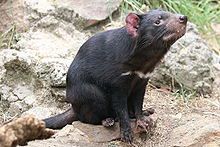
\includegraphics[width=\marginparwidth]{EigGen/TasmanianDevil}
\footnotesize\url{https://en.wikipedia.org/wiki/Tasmanian_devil}}
derive a mathematical model in the form \(\yv(t+1)=A\yv(t)\) for the age structure of the Tasmanian Devil.
By finding eigenvalues and an eigenvector, predict the long-term growth of the population, and predict the long-term relative numbers of Devils of various ages.
\begin{quoted}{Wikipedia, 2016}
Devils are not monogamous, and their reproductive process is very robust and competitive. Males fight one another for the females, and then guard their partners to prevent female infidelity. Females can ovulate three times in as many weeks during the mating season, and 80\%~of two-year-old females are seen to be pregnant during the annual mating season. Females average four breeding seasons in their life and give birth to 20--30 live young after three weeks' gestation. The newborn are pink, lack fur, have indistinct facial features and weigh around 0.20\,g (0.0071\,oz) at birth. As there are only four nipples in the pouch, competition is fierce and few newborns survive. The young grow rapidly and are ejected from the pouch after around 100~days, weighing roughly 200\,g (7.1\,oz). The young become independent after around nine months, so the female spends most of her year in activities related to birth and rearing.
\end{quoted}
\end{exercise}






\begin{exercise} \label{ex:} 
From the following partial description of the \idx{elephant}, 
\marginpar{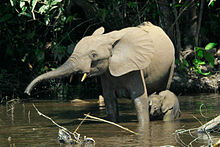
\includegraphics[width=\marginparwidth]{EigGen/Loxodontacyclotis}
\footnotesize\url{https://en.wikipedia.org/wiki/Elephant}}
derive a mathematical model in the form \(\yv(t+1)=A\yv(t)\) for the age structure of the \idx{elephant}.
By finding eigenvalues and an eigenvector, predict the long-term growth of the population, and predict the long-term relative numbers of elephants of various ages.
\begin{quoted}{Wikipedia, 2016}
Gestation in elephants typically lasts around two years with interbirth intervals usually lasting four to five years. Births tend to take place during the wet season. Calves are born 85\,cm (33\,in) tall and weigh around 120\,kg (260\,lb). Typically, only a single young is born, but twins sometimes occur.  The relatively long pregnancy is maintained by five corpus luteums (as opposed to one in most mammals) and gives the foetus more time to develop, particularly the brain and trunk. As such, newborn elephants are precocial and quickly stand and walk to follow their mother and family herd.  A new calf is usually the centre of attention for herd members.  Adults and most of the other young will gather around the newborn, touching and caressing it with their trunks.  For the first few days, the mother is intolerant of other herd members near her young.  Alloparenting---where a calf is cared for by someone other than its mother---takes place in some family groups.  Allomothers are typically two to twelve years old. When a predator is near, the family group gathers together with the calves in the centre.

For the first few days, the newborn is unsteady on its feet, and needs the support of its mother. It relies on touch, smell and hearing, as its eyesight is poor. It has little precise control over its trunk, which wiggles around and may cause it to trip. By its second week of life, the calf can walk more firmly and has more control over its trunk. After its first month, a calf can pick up, hold and put objects in its mouth, but cannot suck water through the trunk and must drink directly through the mouth. It is still dependent on its mother and keeps close to her.

For its first three months, a calf relies entirely on milk from its mother for nutrition after which it begins to forage for vegetation and can use its trunk to collect water.  At the same time, improvements in lip and leg coordination occur.  Calves continue to suckle at the same rate as before until their sixth month, after which they become more independent when feeding.  By nine months, mouth, trunk and foot coordination is perfected.  After a year, a calf's abilities to groom, drink, and feed itself are fully developed.  It still needs its mother for nutrition and protection from predators for at least another year.  Suckling bouts tend to last 2--4\,min/hr for a calf younger than a year and it continues to suckle until it reaches three years of age or older.  Suckling after two years may serve to maintain growth rate, body condition and reproductive ability.  Play behaviour in calves differs between the sexes; females run or chase each other, while males play-fight. The former are sexually mature by the age of nine years while the latter become mature around 14--15 years.  Adulthood starts at about 18~years of age in both sexes.  Elephants have long lifespans, reaching 60--70~years of age.
\end{quoted}
\end{exercise}






\begin{exercise} \label{ex:} 
From the following partial description of the \idx{giant mouse lemur}, 
\marginpar{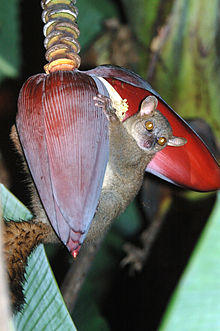
\includegraphics[width=\marginparwidth]{EigGen/Mirza_zaza}
\footnotesize\url{https://en.wikipedia.org/wiki/Giant_mouse_lemur}}
derive a mathematical model in the form \(\yv(t+1)=A\yv(t)\) for the age structure of the \idx{giant mouse lemur}.
By finding eigenvalues and an eigenvector, predict the long-term growth of the population, and predict the long-term relative numbers of \idx{giant mouse lemur}s of various ages.
\begin{quoted}{Wikipedia, 2016}
Reproduction starts in November for Coquerel's giant mouse lemur at Kirindy Forest; the estrous cycle runs approximately 22~days, while estrus lasts only a day or less. \ldots

One to three offspring (typically two) are born after 90~days of gestation, weighing approximately 12\,g (0.42\,oz). Because they are poorly developed, they initially remain in their mother's nest for up to three weeks, being transported by mouth between nests. Once they have grown sufficiently, typically after three weeks, the mother will park her offspring in vegetation while she forages nearby. After a month, the young begin to participate in social play and grooming with their mother, and between the first and second month, young males begin to exhibit early sexual behaviors (including mounting, neck biting, and pelvic thrusting). By the third month, the young forage independently, though they maintain vocal contact with their mother and use a small part of her range.

Females start reproducing after ten months, while males develop functional testicles by their second mating season. Testicle size in the northern giant mouse lemur does not appear to fluctuate by season, and is so large relative to the animal's body mass that it is the highest among all primates. This emphasis on sperm production in males, as well as the use of copulatory plugs, suggests a mating system best described as polygynandrous where males use scramble competition (roaming widely to find many females). In contrast, male Coquerel's giant mouse lemurs appear to fight for access to females (contest competition) during their breeding season. Males disperse from their natal range, and the age at which they leave varies from two years to several. Females reproduce every year, although postpartum estrus has been observed in captivity. In the wild, the lifespan of giant mouse lemurs is thought to rarely exceed five or six years
\end{quoted}
\end{exercise}




\begin{exercise} \label{ex:} 
From the following partial description of the \idx{dolphin} (Indo-Pacific bottlenose dolphin), 
\marginpar{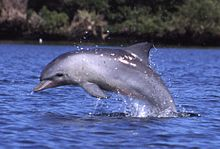
\includegraphics[width=\marginparwidth]{EigGen/Tursiops_aduncus}
\footnotesize\url{https://en.wikipedia.org/wiki/Indo-Pacific_bottlenose_dolphin}}
derive a mathematical model in the form \(\yv(t+1)=A\yv(t)\) for the age structure of the \idx{dolphin}.
(Assume only one calf is born at a time.)
By finding eigenvalues and an eigenvector, predict the long-term growth of the population, and predict the long-term relative numbers of \idx{dolphin}s of various ages.
\begin{quoted}{Wikipedia, 2016}
Indo-Pacific bottlenose dolphins live in groups that can number in the hundreds, but groups of five to 15 dolphins are most common.  In some parts of their range, they associate with the common bottlenose dolphin and other dolphin species, such as the humpback dolphin.

The peak mating and calving seasons are in the spring and summer, although mating and calving occur throughout the year in some regions. Gestation period is about 12~months. Calves are between 0.84 and 1.5~metres (2.8 and 4.9\,ft) long, and weigh between 9 and 21~kilograms (20 and 46\,lb). The calves are weaned between 1.5 and two years, but can remain with their mothers for up to five years. The interbirth interval for females is typically four to six years.

In some parts of its range, this dolphin is subject to predation by sharks; its life span is more than 40 years.
\end{quoted}
\end{exercise}






\begin{exercise} \label{ex:} 
You are given that a mathematical model of the age structure of some animal population is
\begin{eqnarray*}
y_1(t+1)&=& 0.5y_1(t)+y_3(t),\\
y_2(t+1)&=& 0.5y_1(t)+0.7y_2(t),\\
y_3(t+1)&=& 0.3y_2(t)+0.9y_3(t).
\end{eqnarray*}
Invent an animal species, and time scale, and create details of a plausible scenario for the breeding and life cycle of the species that could lead to this mathematical model.  
Write a coherent paragraph about the breeding and life cycle of the species with enough information that someone could deduce this mathematical model from your description.  
Be creative.
\end{exercise}











\begin{exercise} \label{ex:} 
For each of the following matrices, say~\(A\) for instance, find by hand calculation the \idx{eigenvalue}s and \idx{eigenvector}s of the larger matrix~\(\begin{bmatrix} O&A\\\tr A&O \end{bmatrix}\).
Show your working.
Relate these to an \svd\ of the matrix~\(A\).
\begin{parts}
\item \(\eAii=\begin{bmatrix} 3\\4 \end{bmatrix}\)
\answer{\(\lambda=0,\pm5\), \((\frac45,-\frac35,0)\) and \((\frac35,\frac45,\pm1)\)}

\item \(\eAii=\begin{bmatrix} -5&12 \end{bmatrix}\)
\answer{\(\lambda=0,\pm13\), \((0,\frac{12}{13},\frac5{13})\) and \((\pm1,-\frac5{13},\frac{12}{13})\)}

\item \(\eAii=\begin{bmatrix} 1&0\\0&-2 \end{bmatrix}\)
\answer{\(\lambda=\pm1,\pm2\), \((\pm1,0,1,0)\) and \((0,1,0,\mp1)\)}

\item \(\eAii=\begin{bmatrix} 0&1\\-4&0 \end{bmatrix}\)
\answer{\(\lambda=\pm1,\pm4\), \((1,0,0,\pm1)\) and \((0,1,\mp1,0)\)}

\end{parts}
\end{exercise}








\begin{comment}%{ED498555.pdf}
why, what caused X?
how did X occur?
what-if? what-if-not?
how does X compare with Y?
what is the evidence for X?
why is X important?
\end{comment}




